%!TEX root = ../thesis.tex
%*******************************************************************************
%****************************** Second Chapter *********************************
%*******************************************************************************

\chapter{Theoretical Model of Power MEMS Devices}
\label{ch:Theoretical Models of MEMS Cantilever Devices based on AlGaN/AlN/GaN Heterostructure}

\ifpdf
    \graphicspath{{Chapter2/Figs/Raster/}{Chapter2/Figs/PDF/}{Chapter2/Figs/}}
\else
    \graphicspath{{Chapter2/Figs/Vector/}{Chapter2/Figs/}}
\fi


% Uncomment this line, when you have siunitx package loaded.
%The SI Units for dynamic viscosity is \si{\newton\second\per\metre\squared}.

\section{Polarization effects of III-V nitrides}
\label{sec:Polarization effect of III-V nitrides}

III-V nitride \index{Nitride} semiconductor materials usually exhibit very obvious polarization \index{Polarization!effect} effects, namely piezoelectric polarization \index{Piezoelectric!polarization} and \index{Spontaneous polarization} spontaneous polarization. Due to the lack of inversion symmetry centers in semiconducting nitrides, a prominent piezoelectric polarization effect is exhibited when the lattice is strained \index{Strain} along <0001>. The piezoelectric coefficient \index{Piezoelectric!coefficient} in nitrides is almost an order of magnitude larger than many conventional III-V semiconductors \cite{bykhovski1993influence,bykhovski1997elastic,gualtieri1994piezoelectric,o1973acoustic}. The piezoelectric polarization effect has two components, one is lattice strain \index{Lattice!strain} caused by lattice mismatch \index{Lattice!mismatch} between the substrate \index{Substrate} and the epitaxial layer \index{Epitaxial!layer} and the other is thermal strain caused by the difference in thermal expansion coefficient between the substrate \index{Substrate} and the \index{Epitaxial!layer} epitaxial layer. Furthermore, due to the low symmetry of nitrides, there is a spontaneous polarization \index{Spontaneous polarization} effect in ideal \index{Wurtzite} wurtzite-structured nitrides, which induces intrinsic spontaneously polarized charges at the material \index{Surface} surface \cite{resta1994macroscopic,king1993theory}. Especially when involving the heterojunction interface \index{Interface} between two nitride semiconductors with different \index{Electronegativity} electronegativities, the spontaneous polarization charge at the heterojunction interface caused by the spontaneous polarization effect can significantly modulate the heterojunction energy band \index{Energy band} and optoelectronic properties.

Due to polarization effects in III-V nitride \index{Nitride} semiconductor materials, there is a high density of polarization charges \index{Polarization!charge} at the interface \index{Interface} of heterojunction devices with significant lattice strain \index{Lattice!strain} (such as HEMTs), and polarization charges \index{Polarization!charge} are closely related to the energy \index{Energy band} band, free carrier distribution \index{Carrier!distribution} and density in the heterojunction. Therefore, polarization effects \index{Polarization!effect} affect the performance of all nitride-based semiconductor devices, especially \index{HEMT} HEMTs. Unless using non-polar surfaces \index{Surface} (such as a-planes), material polarization effects must be considered in device design. Taking the AlGaN/AlN/GaN \index{AlGaN/AlN/GaN heterojunction} heterojunction as an example, as mentioned above, in the absence of external \index{Strain} strain, the polarization charge at the interface \index{Interface} of the heterojunction has two origins: the piezoelectric polarization \index{Piezoelectric!polarization charge} charge ($P_{PE}$) caused by lattice mismatch \index{Lattice!mismatch} between films, and the spontaneous polarization \index{Spontaneous polarization} charge ($P_{SP}$) of the film itself. Generally the spontaneous polarization in the AlGaN/AlN/GaN heterojunction is larger than the piezoelectric polarization in the absence of external strain, and the strain in the heterojunction film decreases when defect-related relaxation occurs, resulting in a weakening of the \index{Piezoelectric!polarization} piezoelectric polarization. These polarized charges are present to varying degrees in all III-V nitride \index{Nitride} semiconductors unless counteracted by considering lattice symmetry in a particular direction (eg, non-polar surfaces). Since the spontaneous polarization and piezoelectric polarization charges in III-V nitride semiconductor materials can significantly affect the energy band \index{Energy band} of the heterojunction, thereby changing the optoelectronic properties of the heterojunction, the electrical performance of AlGaN/AlN/GaN \index{AlGaN/AlN/GaN heterojunction} MEMS \index{MEMS} can be effectively modulated by artificially changing the piezoelectric polarization charge in the material \cite{kim2013polarization,jena2011polarization,verma2018polarization}.

The polarization effect \index{Polarization!effect} depends on the polarity of the \index{Crystal} crystal. For GaN crystals, the $[0001]$ oriented crystals are called Ga polar crystals, and the $[000\overline{1}]$ oriented crystals are called N polar crystals. It is worth noting that polarity is a bulk property of a material, not a surface \index{Surface} property. One can imagine a situation in which N-polar GaN is covered by a monolayer of Ga, but the orientation and polarity of the crystal \index{Crystal} remain unchanged. Therefore, the polarity of GaN can usually be judged by the following way. When the bond (single bond) along the c-direction of the crystal is from $Ga^{+}$ ion to $N^{-}$ ion, the polarity is called Ga polarity. Similarly, when the bonds (single bonds) in the c-direction of the crystal are from $N^{-}$ ions to $Ga^{+}$ ions, the polarity is called N-polarity. Briefly, Ga-polar crystals mean that if the crystal is cut along the c-plane, but only a single bond of the tetrahedral lattice is broken, the surface of the final crystal is a Ga-plane. The opposite is true for N-polar crystals. Studies have shown that the polarity faces of III-V nitride \index{Nitride} semiconductor materials have a significant impact on heterojunction energy band \cite{jang2002characterization}, 2DEG concentration \cite{dimitrov2000two}, electrical properties \cite{guerra2010comparison,dimitrov1999comparison}, short channel effect \cite{park2011simulation}, and light reflection \cite{buchheim2004photoreflectance}, and other optoelectronic properties.

\begin{figure}[H] 
\centering    
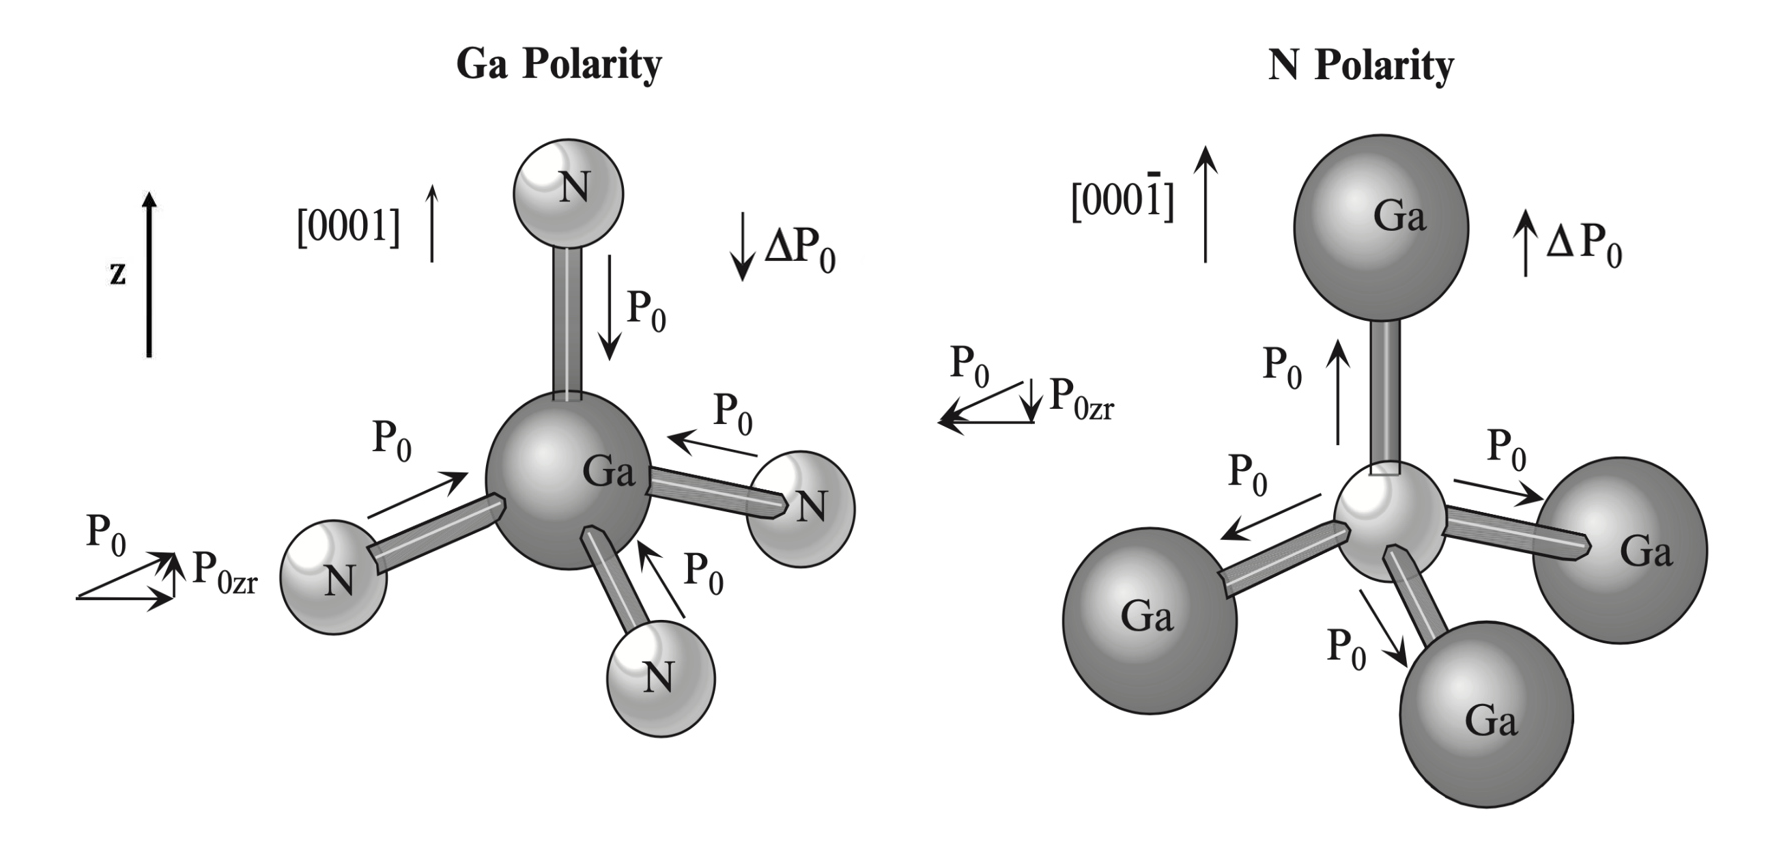
\includegraphics[width=0.9\textwidth]{ch2_1}
\caption[Ball and stick model of an ideal GaN crystal with Ga and N-polarity in a relaxed state]{Ball and stick model of an ideal GaN crystal with Ga and N-polarity in a relaxed state \protect\cite{morkoc2008polarization}}
\label{fig:2.1}
\end{figure}

The effects of polarization due to the low symmetry of the lattice (spontaneous \index{Spontaneous polarization} polarization) and the lattice strain \index{Lattice!strain} of the heterojunction interface \index{Interface} (piezoelectric \index{Piezoelectric!polarization} polarization) can be visualized by the simplified ball and stick model. Shown in \autoref{fig:2.1} is a ball-and-stick diagram of the tetrahedral lattice between $Ga$ ions and $N$ ions in the relaxed Ga-polar and N-polar 

\begin{figure}[H] 
\centering    
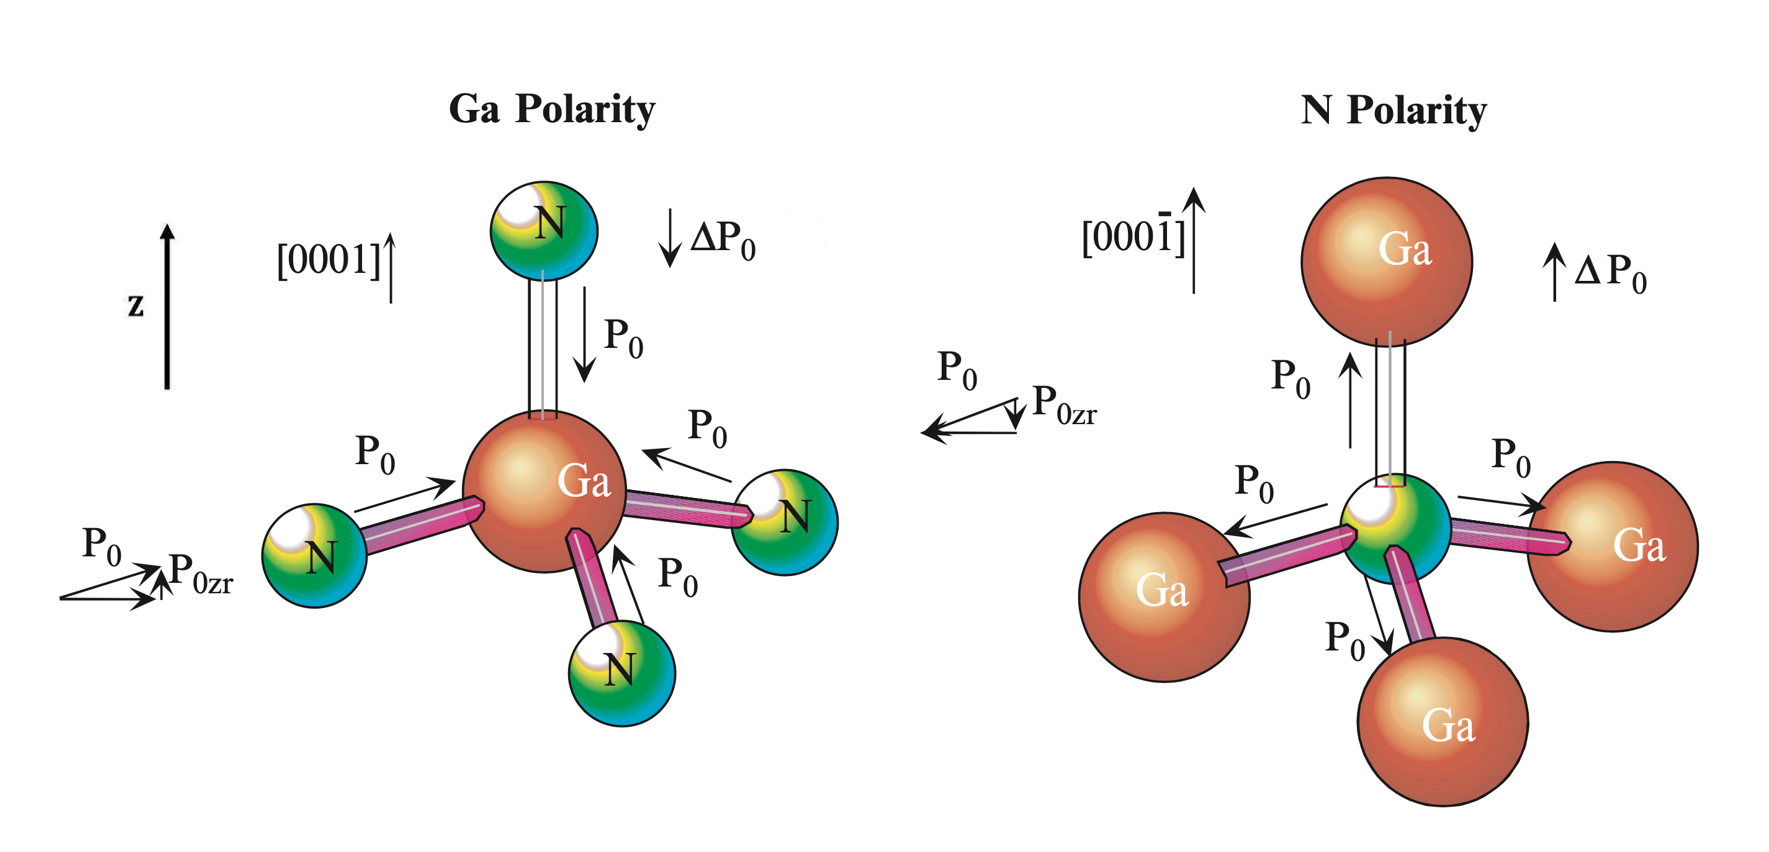
\includegraphics[width=0.9\textwidth]{ch2_2}
\caption[Ball and stick model of a GaN crystal for both Ga and N polarity with a homogeneous in-plane tensile strain]{Ball and stick model of a GaN crystal for both Ga and N polarity with a homogeneous in-plane tensile strain \protect\cite{morkoc2008polarization}}
\label{fig:2.2}
\end{figure}

\begin{figure}[H] 
\centering    
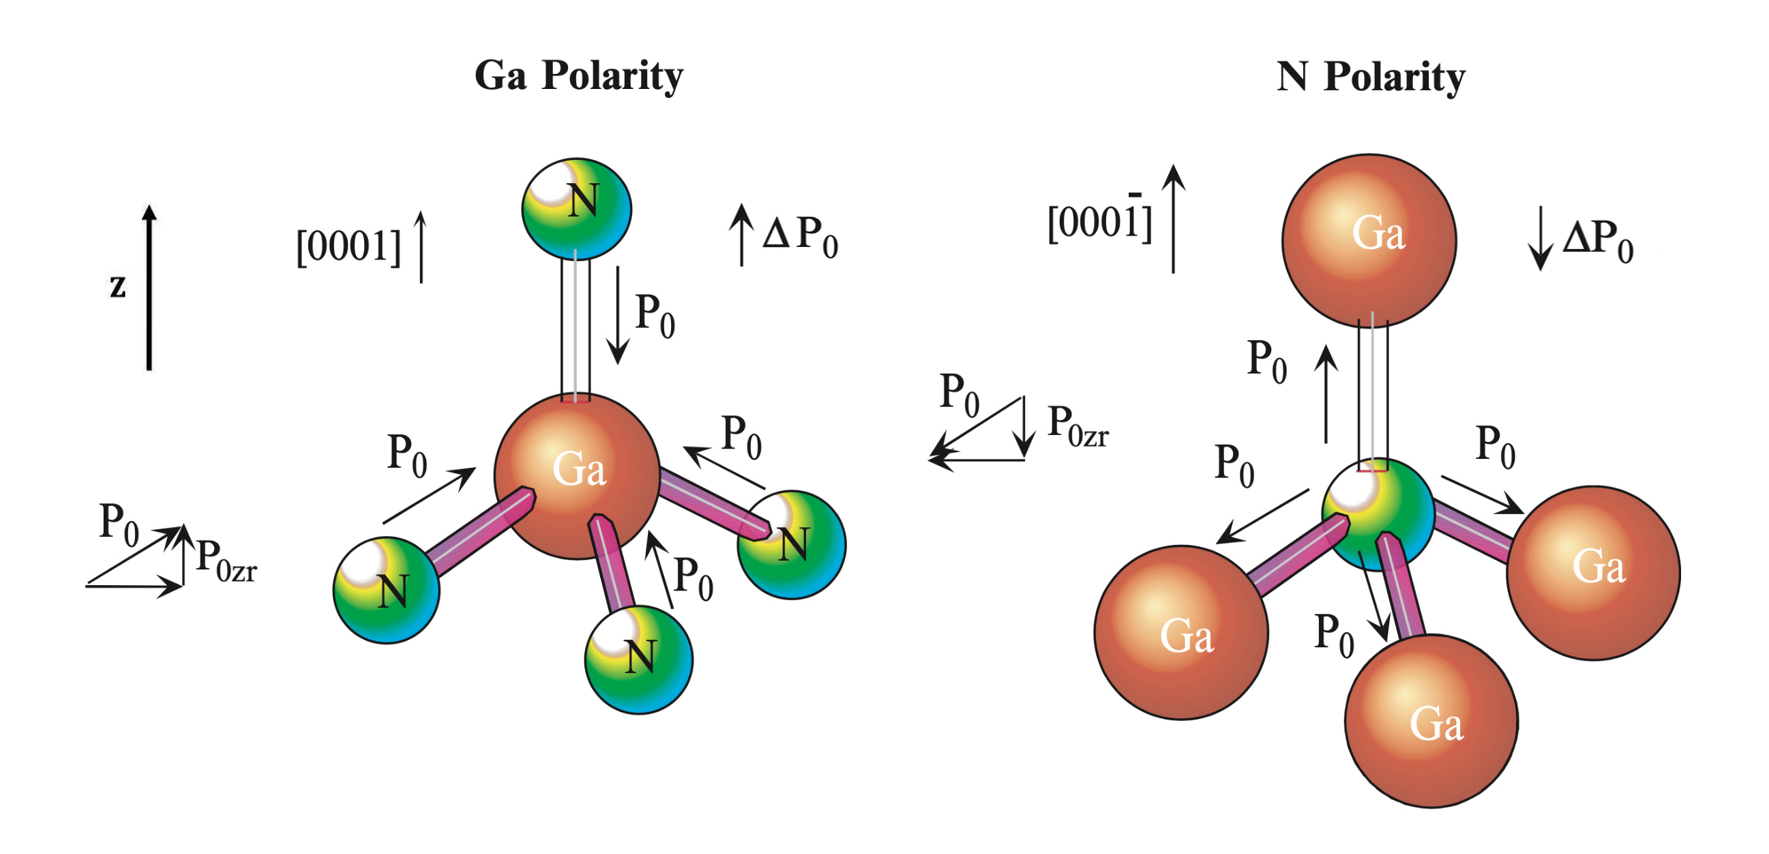
\includegraphics[width=0.9\textwidth]{ch2_3}
\caption[Ball and stick model of a GaN crystal for both Ga and N polarity with a homogeneous in-plane compressive strain]{Ball and stick model of a GaN crystal for both Ga and N polarity with a homogeneous in-plane compressive strain \protect\cite{morkoc2008polarization}}
\label{fig:2.3}
\end{figure}

\noindent GaN lattices, where $P_{0}$ denotes the pole between $Ga$ ions and $N$ ions vectorization. Take the GaN lattice with Ga polarity in the left figure as an example, since the electron cloud of the lattice is closer to the N atom, in the tetrahedral structure, the superposition of the \index{Polarization!vector} polarization vector $P_{0zr}$ in the $+z$ direction of the three bonds of the tetrahedral lattice cannot cancel it out. The polarization vector $P_{0}$ in the $-z$ direction, so the net polarization vector of the Ga-polar GaN lattice is along the $-z$ direction. The net polarization phenomenon in this lattice relaxation state is the spontaneous polarization \index{Spontaneous polarization} effect. However, when the Ga-polar GaN lattice is under uniform in-plane tensile strain, the accumulated polarization vector \index{Polarization!vector} in the $+z$ direction associated with the three bonds of the tetrahedral lattice decreases, thereby enhancing the net polarization vector along the $-z$ direction, as shown in \autoref{fig:2.2}. When there is in-plane uniform compressive strain in the Ga-polar GaN lattice, the cumulative polarization vector \index{Polarization!vector} in the $+z$ direction related to the three bonds of the tetrahedral lattice will increase, and the GaN lattice exhibits a net polarization vector along the $+z$ direction, as shown in \autoref{fig:2.3}. The change of the polarization vector in this external stress state is called the piezoelectric polarization \index{Piezoelectric!polarization} effect, and the change of net polarization vector of the lattice is the result of the combined action of the spontaneous polarization \index{Spontaneous polarization} and the piezoelectric polarization. In an N-polar GaN lattice, the same happens, except that the polarization direction is opposite to that of a Ga-polar GaN lattice \cite{morkoc2008polarization}.


\section{Piezoelectric theory of III-V nitrides}
\label{sec:Piezoelectric equations for III-V nitrides}
\subsection{Piezoelectric constitutive equation}
\label{sec:Piezoelectric constitutive equation}

According to the basic theory of piezoelectric \index{Piezoelectric!effect} effect, the stress-charge form of piezoelectric constitutive equation \index{Piezoelectric!constitutive equation} can be expressed as
\begin{equation}
\left\{\begin{array}{c}
\boldsymbol{\sigma}=\boldsymbol{c}_{E} \boldsymbol{S}-\boldsymbol{e}^{T} \boldsymbol{E} \\
\boldsymbol{D}=\boldsymbol{e} \boldsymbol{S}+\boldsymbol{k} E
\end{array}\right.
\label{eq:2.1}
\end{equation}
In this formula, $\boldsymbol{E}$ and $\boldsymbol{D}$ represent the electric \index{Electric!field} field strength vector and \index{Electric!displacement vector} electric displacement vector, and $\sigma$ is the stress tensor; $\boldsymbol{c}_{E}$ is the \index{Elastic!coefficient} elastic coefficient tensor; $\boldsymbol{e}$ is the linear piezoelectric \index{Piezoelectric!coefficient} coefficient; $\boldsymbol{k}$ is the dielectric constant tensor, and $\boldsymbol{S}$ is the strain \index{Strain} tensor.
Among them, the expression of linear \index{Piezoelectric!coefficient} piezoelectric coefficient $\boldsymbol{e}$ is
\begin{equation}
\boldsymbol{e}=\begin{bmatrix}
e_{11} & e_{12} & e_{13} & e_{14} & e_{15} & e_{16} \\
e_{21} & e_{22} & e_{23} & e_{24} & e_{25} & e_{26} \\
e_{31} & e_{32} & e_{33} & e_{34} & e_{35} & e_{36}
\end{bmatrix}
\label{eq:2.2}
\end{equation}
Next, we start to simplify the theoretical model. First, we only consider the condition of the external \index{Electric!field} electric field $\boldsymbol{E} = 0$. Therefore, \autoref{eq:2.1} can be simplified as
\begin{equation}
\left\{\begin{array}{c}
\boldsymbol{\sigma}=\boldsymbol{c}_{E} \boldsymbol{S}\\
\boldsymbol{D}=\boldsymbol{e} \boldsymbol{S}
\end{array}\right.
\label{eq:2.3}
\end{equation}
Since we only need to study the \index{Piezoelectric!polarization charge} piezoelectric polarization charge-strain \index{Strain} relationship, we only take $\boldsymbol{D}=\boldsymbol{e} \boldsymbol{S}$ for discussion, and the thin film \index{Thin film} materials we study are the III-V group nitride materials AlGaN, AlN and GaN with wurtzite \index{Wurtzite} structure. The linear piezoelectric \index{Piezoelectric!coefficient} coefficient $\boldsymbol{e}$ matrix has a special form, and its expansion is written in the matrix form as
\begin{equation}
\begin{bmatrix}
D_{x} \\
D_{y} \\
D_{z}
\end{bmatrix}=\begin{bmatrix}
0 & 0 & 0 & 0 & e_{15} & 0 \\
0 & 0 & 0 & e_{24} & 0 & 0 \\
e_{31} & e_{32} & e_{33} & 0 & 0 & 0
\end{bmatrix}\begin{bmatrix}
S_{x x} \\
S_{y y} \\
S_{z z} \\
S_{y z} \\
S_{x z} \\
S_{x y}
\end{bmatrix}
\label{eq:2.4}
\end{equation}
where $𝑒_{31} = 𝑒_{32}$. Since we only study the \index{Piezoelectric!polarization charge} piezoelectric polarization charge-strain \index{Strain} relationship in the $z$ direction, ie $D_{z}$, from \autoref{eq:2.4} we can get
\begin{equation}
\begin{aligned}
D_{z} &=e_{31} S_{x x}+e_{32} S_{y y}+e_{33} S_{z z} \\
&=e_{31}\left(S_{x x}+S_{y y}\right)+e_{33} S_{z z}
\end{aligned}
\label{eq:2.5}
\end{equation}
Therefore, the $z$-direction \index{Electric!displacement vector} electric displacement vector-strain \index{Strain} equation of III-V nitride \index{Nitride} materials is derived from the piezoelectric \index{Piezoelectric!constitutive equation} constitutive equation, where $S_{x x}$, $S_{y y}$, $S_{z z}$ are the strains of the material in the $x$, $y$, and $z$ directions, respectively.

\subsection{Piezoelectric polarization charge-strain equation}
\label{sec:Piezoelectric polarization-strain equation}

In electromagnetism, the electric displacement vector and electric polarization intensity are defined as:
\begin{equation}
\mathbf{D}=\varepsilon_{0} \mathbf{E}+\mathbf{P}
\label{eq:2.6}
\end{equation}
where $\mathbf{D}$ is the electric displacement \index{Electric!displacement vector} vector, $\varepsilon_{0}$ is the \index{Vacuum permittivity} vacuum permittivity, $\mathbf{E}$ is the electric field \index{Electric!field} strength, and $\mathbf{P}$ is the electric polarization \index{Electric!polarization strength} strength.

Since we only consider the condition of the external electric field \index{Electric!field} $\mathbf{E}=0$, and only consider the electric polarization in the z direction, \autoref{eq:2.6} can be simplified as:
\begin{equation}
D_{z}=P_{z}
\label{eq:2.7}
\end{equation}
Substituting it into \autoref{eq:2.5}, we finally get the \index{Piezoelectric!polarization charge} piezoelectric polarization charge-strain \index{Strain} equation in the $z$-direction of III-V nitride \index{Nitride} materials:
\begin{equation}
P_{z} =e_{31}\left(S_{x x}+S_{y y}\right)+e_{33} S_{z z}
\label{eq:2.8}
\end{equation}

Next, we discuss the physical meaning of \autoref{eq:2.8} in this study. The electric polarization \index{Electric!polarization strength} strength $\mathbf{P}$ (or electric polarization, or simply polarization) is the vector field that represents the density of permanent electric dipole moment \index{Electric!dipole moment} or induced electric dipole moment in the dielectric material, and is a physical quantity characterizing electric dipole moment in a material. In III-V nitride \index{Nitride} materials, the electric polarization $\mathbf{P}$ defined by \autoref{eq:2.8} can characterize the piezoelectric polarization \index{Piezoelectric!polarization} in the $z$ direction $P_{z}$ induced by \index{Strain} strain, so is usually represented by $P_{PE}$, \autoref{eq:2.8} is further rewritten for
\begin{equation}
P_{PE} =e_{31}\left(S_{x x}+S_{y y}\right)+e_{33} S_{z z}
\label{eq:2.9}
\end{equation}

So far, we have derived the mathematical equation for the relationship between piezoelectric polarization \index{Piezoelectric!polarization} and strain \index{Strain} in the $z$-direction of III-V nitride \index{Nitride} materials. When $P_{PE}< 0$, the polarization electric field \index{Polarization!electric field} in the material points to the negative direction of the $z$-axis, and is is directed from negative charges to positive charges. The distribution of piezoelectric polarization charges \index{Piezoelectric!polarization charge} is shown in \autoref{fig:2.4}. Conversely, when $P_{PE} > 0$, the polarization electric field in the material points in the positive z-axis direction, and the distribution of piezoelectric polarization charges is opposite to that in \autoref{fig:2.4}.

\begin{figure}[H] 
\centering    
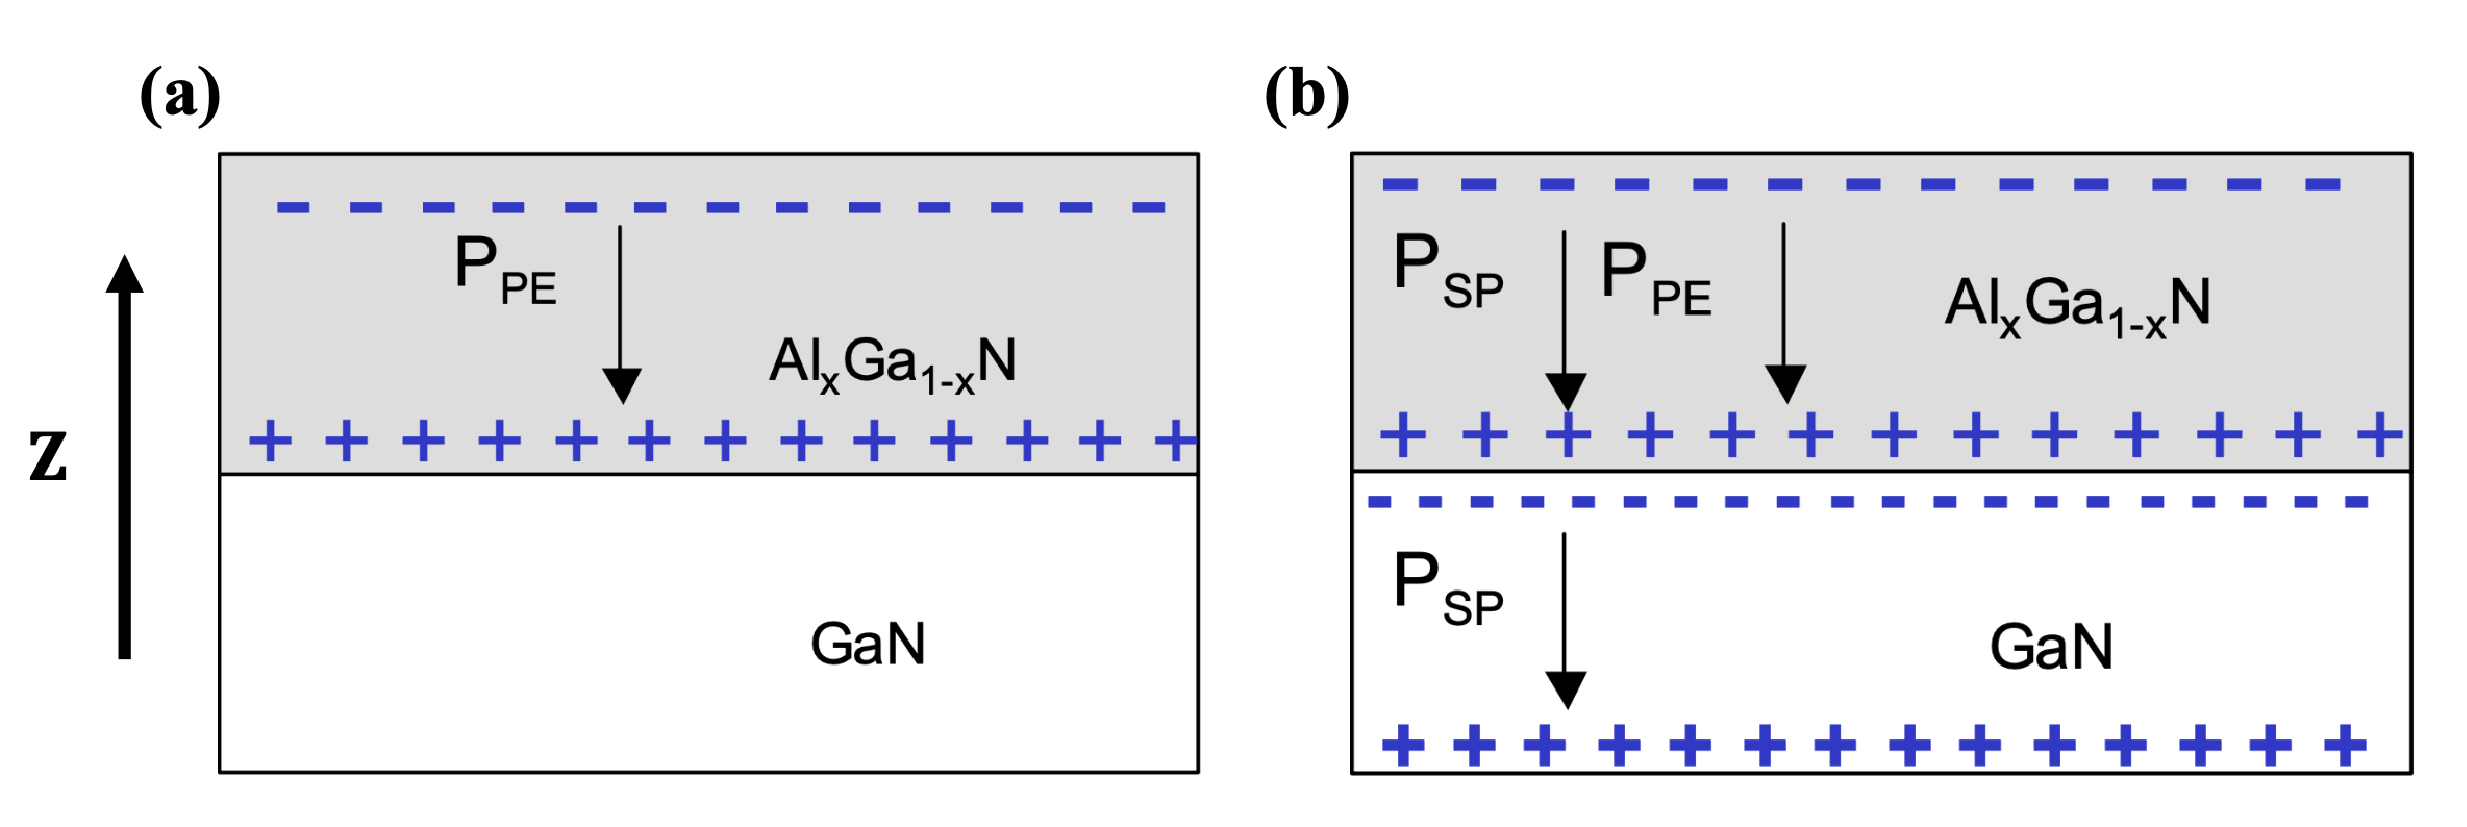
\includegraphics[width=0.9\textwidth]{ch2_4}
\caption[Piezoelectric polarization charge distribution of group III-V nitride material $Al_{x}Ga_{1-x}N$ when $P_{PE}<0$]{Piezoelectric polarization charge distribution of group III-V nitride material $Al_{x}Ga_{1-x}N$ when $P_{PE}<0$. (a) Spontaneous polarization charge is not considered. (b) Spontaneous polarization charge is considered \protect\cite{vetury2000polarization}}
\label{fig:2.4}
\end{figure}

\section{Lattice strain model of AlGaN/AlN/GaN heterojunction}
\label{sec:Lattice strain model of AlGaN/AlN/GaN heterojunction}

\subsection{Biaxial strain model of thin films}
\label{sec:Biaxial strain model of thin films}

In this section, we study the strains \index{Strain} of \index{AlGaN/AlN/GaN heterojunction} AlGaN/AlN/GaN heterojunction thin films \index{Thin film} in the $x$, $y$, and $z$ directions. The thicknesses of the AlGaN, AlN, and GaN films are 30 \unit{nm}, 1 \unit{nm}, and 4.3 \unit{um}, respectively. The thickness of the GaN film is much larger than AlGaN thin film \index{Thin film} and AlN thin film, and the GaN material is rigid. Therefore, we can approximately think that the GaN thin film is a rigid substrate \index{Substrate} material, and use the biaxial stress model \index{Biaxial stress model} to perform strain \index{Strain} analysis on the AlGaN thin film and the AlN thin film, as shown in \autoref{fig:2.5}. The thickness of the film material is much smaller than that of the rigid substrate, so when the film is subjected to lateral strain, the axial strain of the film can be calculated approximately through the Poisson's ratio \index{Poisson's!ratio} of the material:
\begin{equation}
S_{z}=-\frac{v}{1-v}\left(S_{x}+S_{y}\right)
\label{eq:2.10}
\end{equation}
where $S_{x}$, $S_{y}$, $S_{z}$ are the strains \index{Strain} in the $x$, $y$, and $z$ directions, respectively, and $v$ is the Poisson's ratio \index{Poisson's!ratio} of the thin film \index{Thin film} material.

\begin{figure}[H] 
\centering    
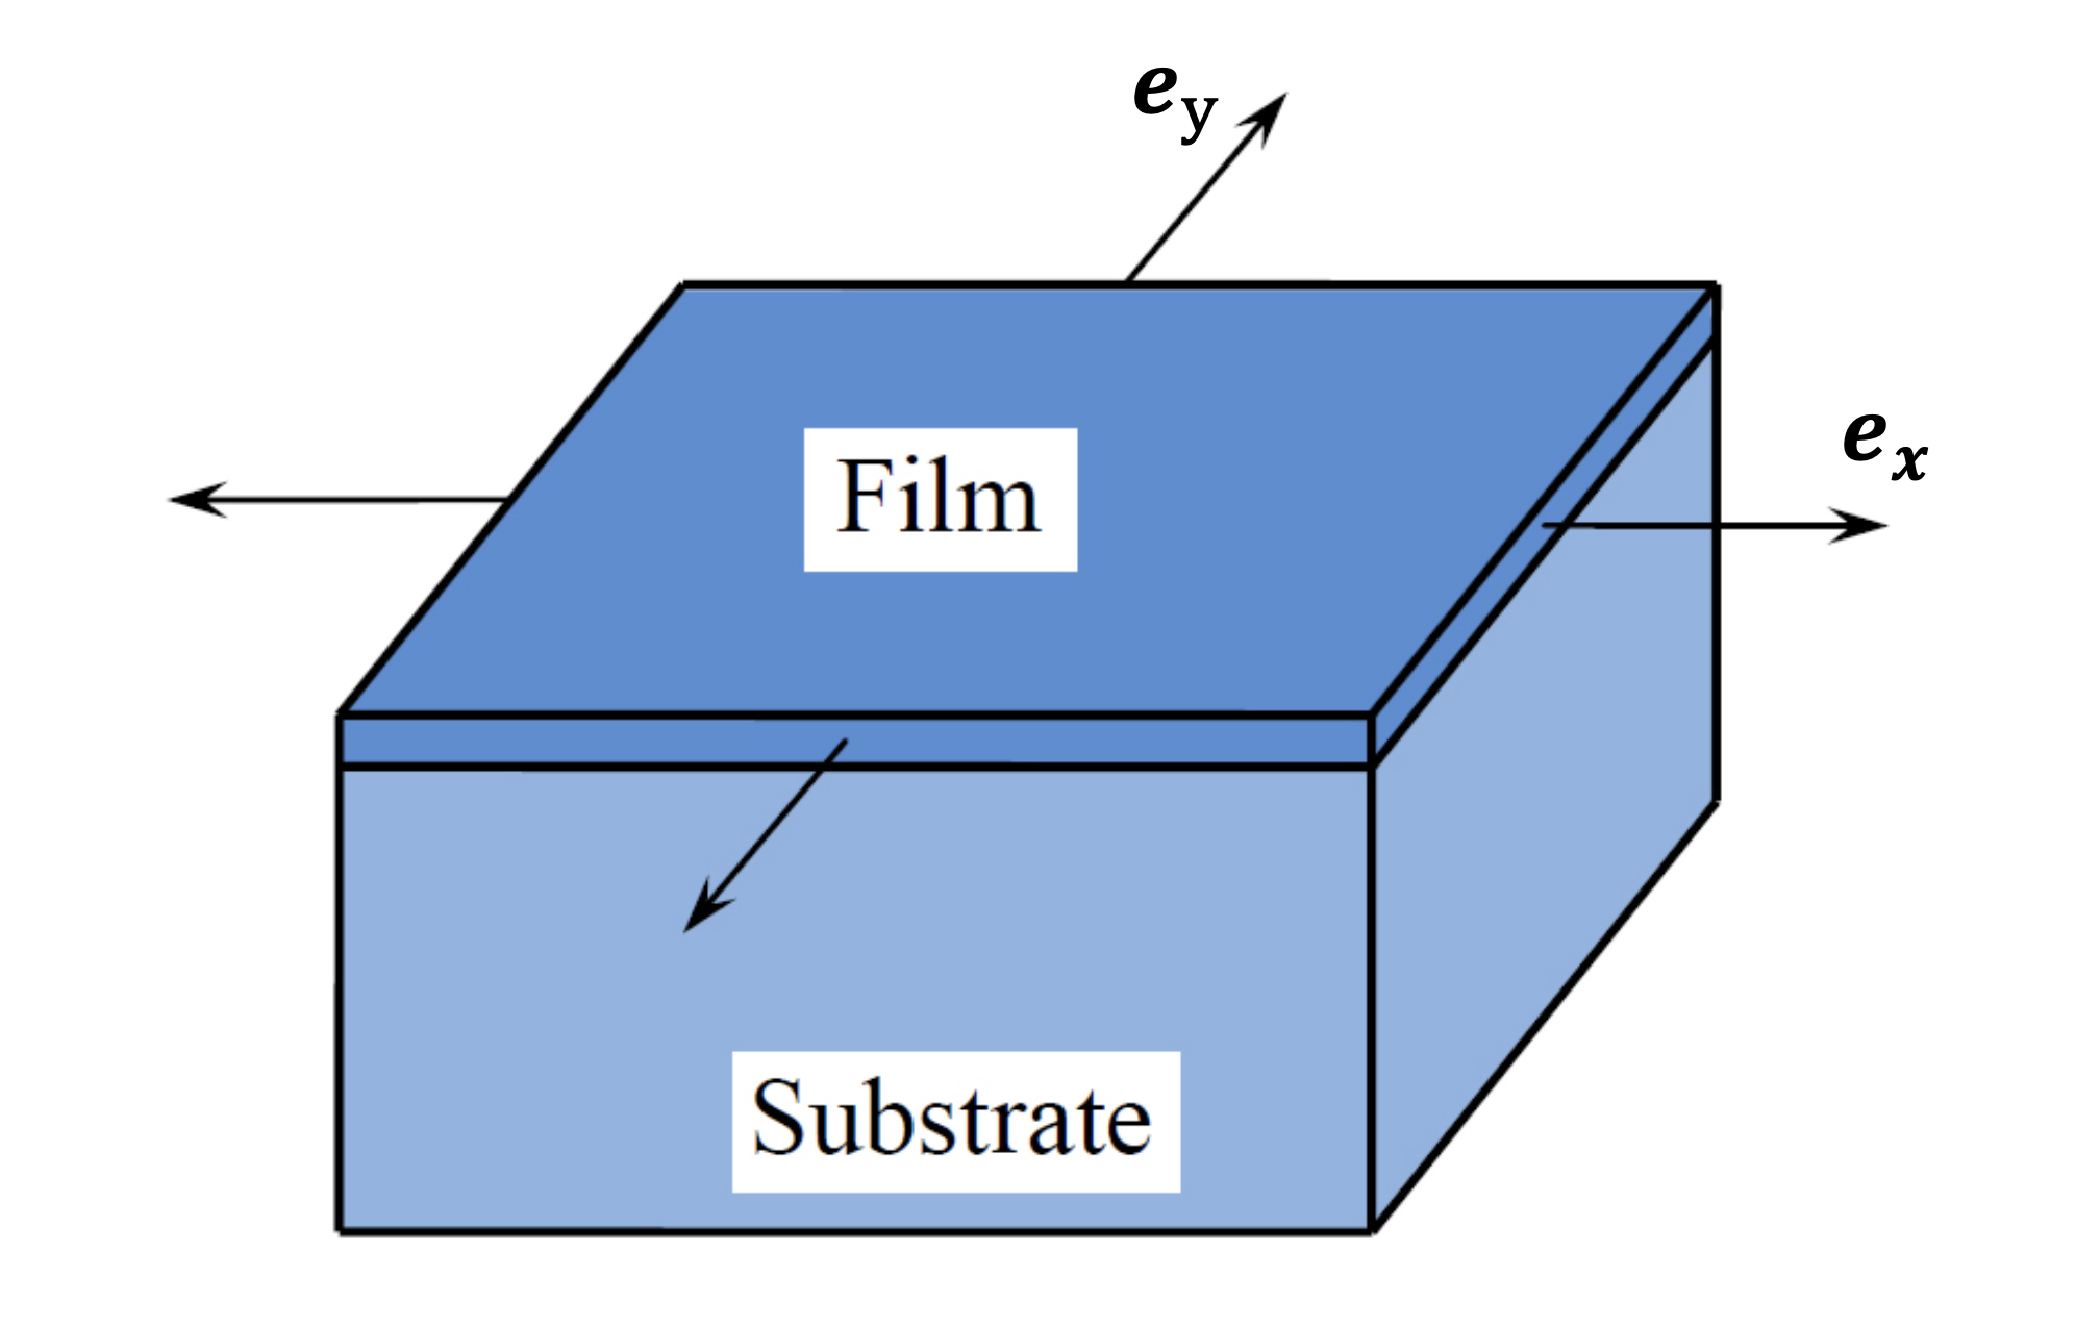
\includegraphics[width=0.6\textwidth]{ch2_5}
\caption[Schematic diagram of biaxial stress model]{Schematic diagram of biaxial stress model}
\label{fig:2.5}
\end{figure}

\subsection{Lattice strain in multilayer thin films}
\label{sec:Lattice strain in multilayer thin films}

Next we investigate the lattice strain \index{Lattice!strain} of the thin film \index{Thin film} due to \index{Lattice!mismatch} lattice mismatch. \autoref{fig:2.6} shows the relationship between the forbidden band width and lattice constant \index{Lattice!constant} of III-V nitride \index{Nitride} semiconductors at room temperature, where the lattice constant \index{Lattice!constant} of AlGaN (30$\%\;$Al) can be given by Vegard's law \index{Vegard's law} \cite{vegard1921konstitution,denton1991vegard}:
\begin{equation}
a_{\mathrm{Al}_{0.3} \mathrm{Ga}_{0.7 \mathrm{~N}}}=0.3 a_{\mathrm{AlN}}+0.7 a_{\mathrm{GaN}}
\label{eq:2.11}
\end{equation}
We can see that the lattice constants \index{Lattice!constant} of AlN crystal, AlGaN crystal and GaN crystal \index{Crystal} are inconsistent, and there is a certain lattice mismatch \index{Lattice!mismatch} between them. It is the lattice mismatch between the thin films \index{Thin film} in the \index{AlGaN/AlN/GaN heterojunction} AlGaN/AlN/GaN heterojunction that introduces strain \index{Strain} in the films, resulting in the corresponding piezoelectric polarization charge. It is also called lattice strain \index{Lattice!strain} because this strain is caused by lattice mismatch.

\begin{figure}[H] 
\centering    
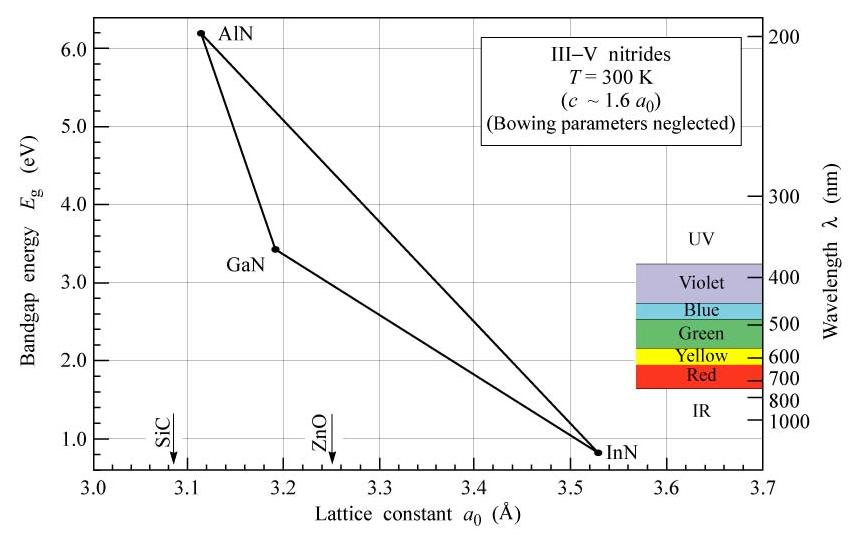
\includegraphics[width=0.9\textwidth]{ch2_6}
\caption[Bandgap energy versus lattice constant for III-V nitride semiconductors at room temperature
]{Bandgap energy versus lattice constant for III-V nitride semiconductors at room temperature}
\label{fig:2.6}
\end{figure}

The lattice strain \index{Lattice!strain} of the \index{Thin film} thin film is shown in \autoref{fig:2.7}. Due to the inconsistency of \index{Lattice!constant} lattice constants, crystals $A$ and $B$ have \index{Crystal} a certain lattice \index{Lattice!mismatch} mismatch. When the epitaxial layer \index{Epitaxial!layer} is composed of these two crystal materials, under ideal conditions (without considering the lattice-mismatched dislocations) there will be elastic strains \index{Elastic!strain} between lattices. Usually, since the thickness of the epitaxial substrate is much larger than that of the \index{Thin film} thin film, we approximately think that the lattice of the substrate \index{Substrate} does not produce \index{Elastic!strain} elastic strain, that is, the \index{Lattice!constant} lattice constant $a_{A}$ of the substrate $A$ does not change, and the lattice of the thin film $B$ undergoes \index{Elastic!deformation} elastic \index{Deformation} deformation. Thus, the deformed lattice constant \index{Lattice!constant} $a_{B}(epi)$ is equal to the lattice constant $a_{A}$ of the substrate $A$, that is, $a_{B}(epi)=a_{A}$. Then, the lateral lattice \index{Lattice!strain} strain $S_{B}$ of film $B$ is:
\begin{equation}
\begin{aligned}
S_{B} &=\frac{a_{B}(e p i)-a_{B}}{a_{B}} \\
&=\frac{a_{A}-a_{B}}{a_{B}}
\end{aligned}
\label{eq:2.12}
\end{equation}
In the ideal case of no external stress, the lateral $x$- and $y$-direction lattice strains \index{Lattice!strain} of film B are approximately the same, and the $z$-direction lattice strain \index{Lattice!strain} can be obtained according to the biaxial stress model \index{Biaxial stress model} (\autoref{eq:2.10}).

\begin{figure}[H] 
\centering    
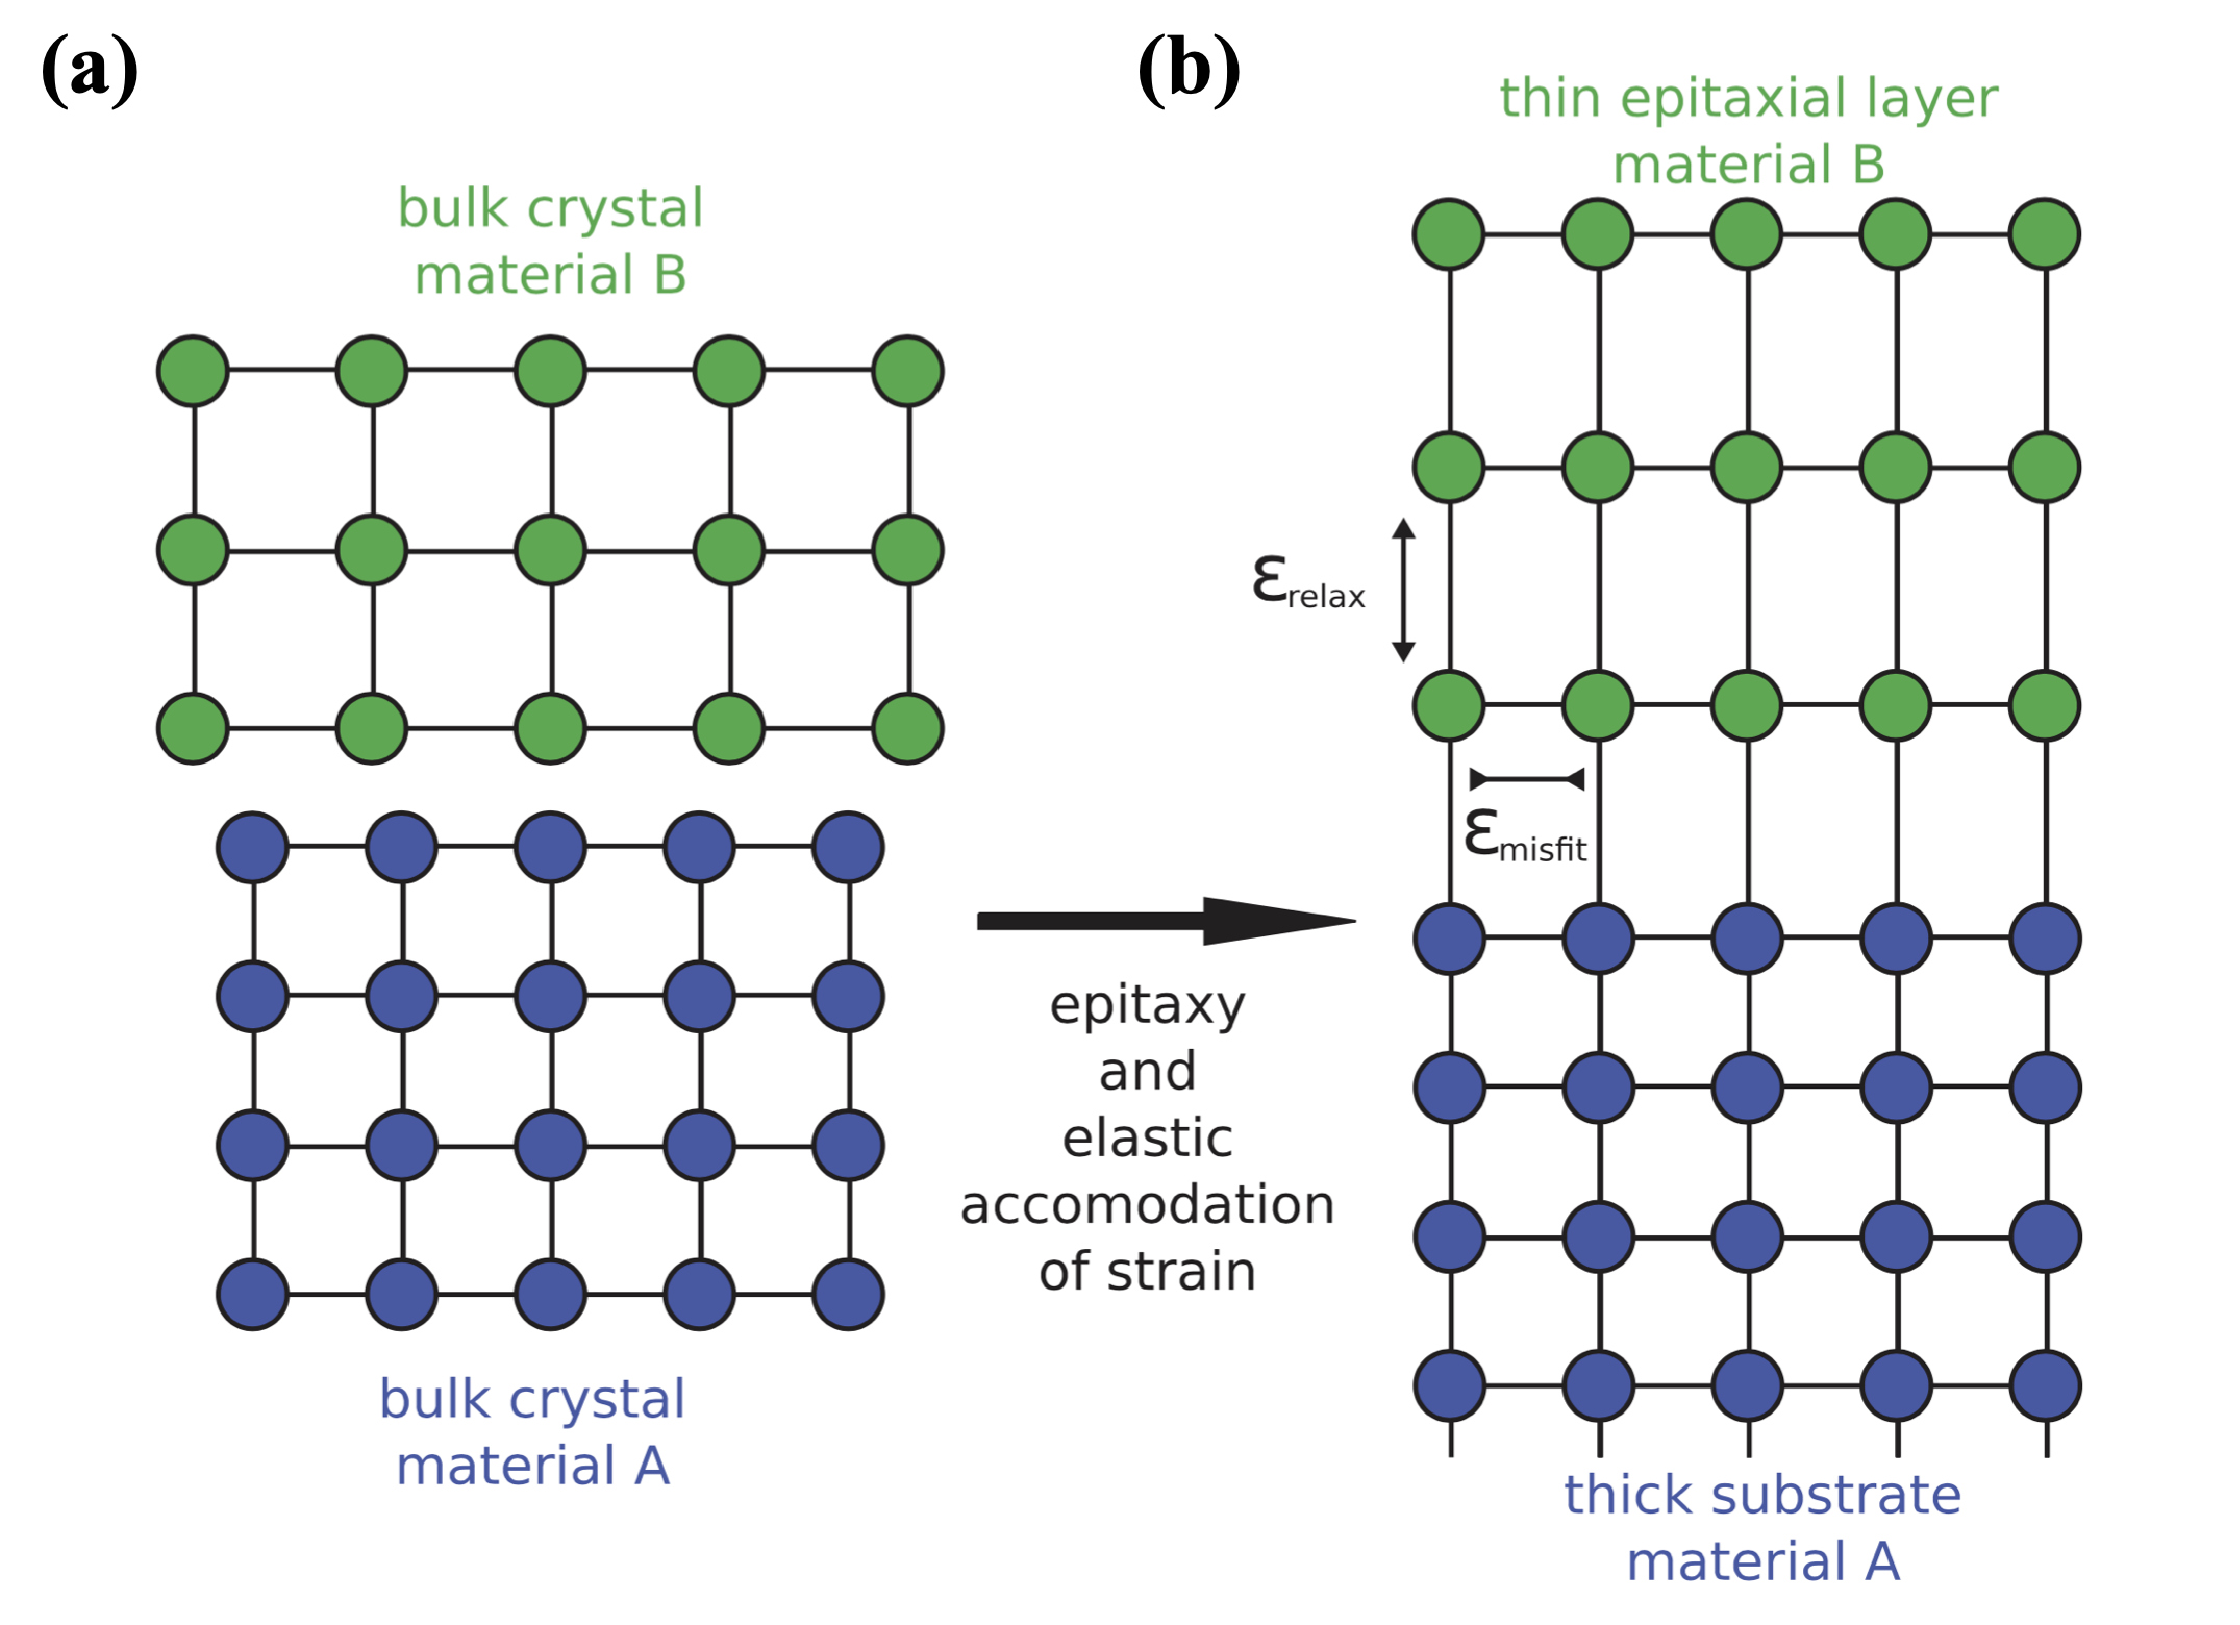
\includegraphics[width=0.9\textwidth]{ch2_7}
\caption[Lattice strain of the thin films]{Lattice strain of the thin films (a) Lattice mismatch between film and substrate material. (b) Purely elastic strain epitaxial layer without misfit dislocations \protect\cite{lopuszynski2012ordering}}
\label{fig:2.7}
\end{figure}

Similarly, considering the \index{AlGaN/AlN/GaN heterojunction} AlGaN/AlN/GaN heterojunction in this study and the thickness of each layer material (30 \unit{nm}/1 \unit{nm}/4.3 \unit{um}), the thickness of the GaN layer is much larger than that of the AlN film and the AlGaN film, We can approximate that GaN belongs to rigid substrate \index{Substrate} materials, and AlN and AlGaN belong to \index{Thin film} thin film materials. This is a structure consisting of two thin films, as shown in \autoref{fig:2.8}. It can be seen that since the lattice constants \index{Lattice!constant} of AlN crystal and AlGaN crystal \index{Crystal} are both smaller than those of GaN crystal, and the thickness of the GaN layer is much larger than that of the AlN film and the AlGaN film, the AlN film and AlGaN film are both subjected to tensile strain, and the lattice constants after deformation \index{Deformation} are all equal to lattice constants of GaN crystals.

\begin{figure}[H] 
\centering    
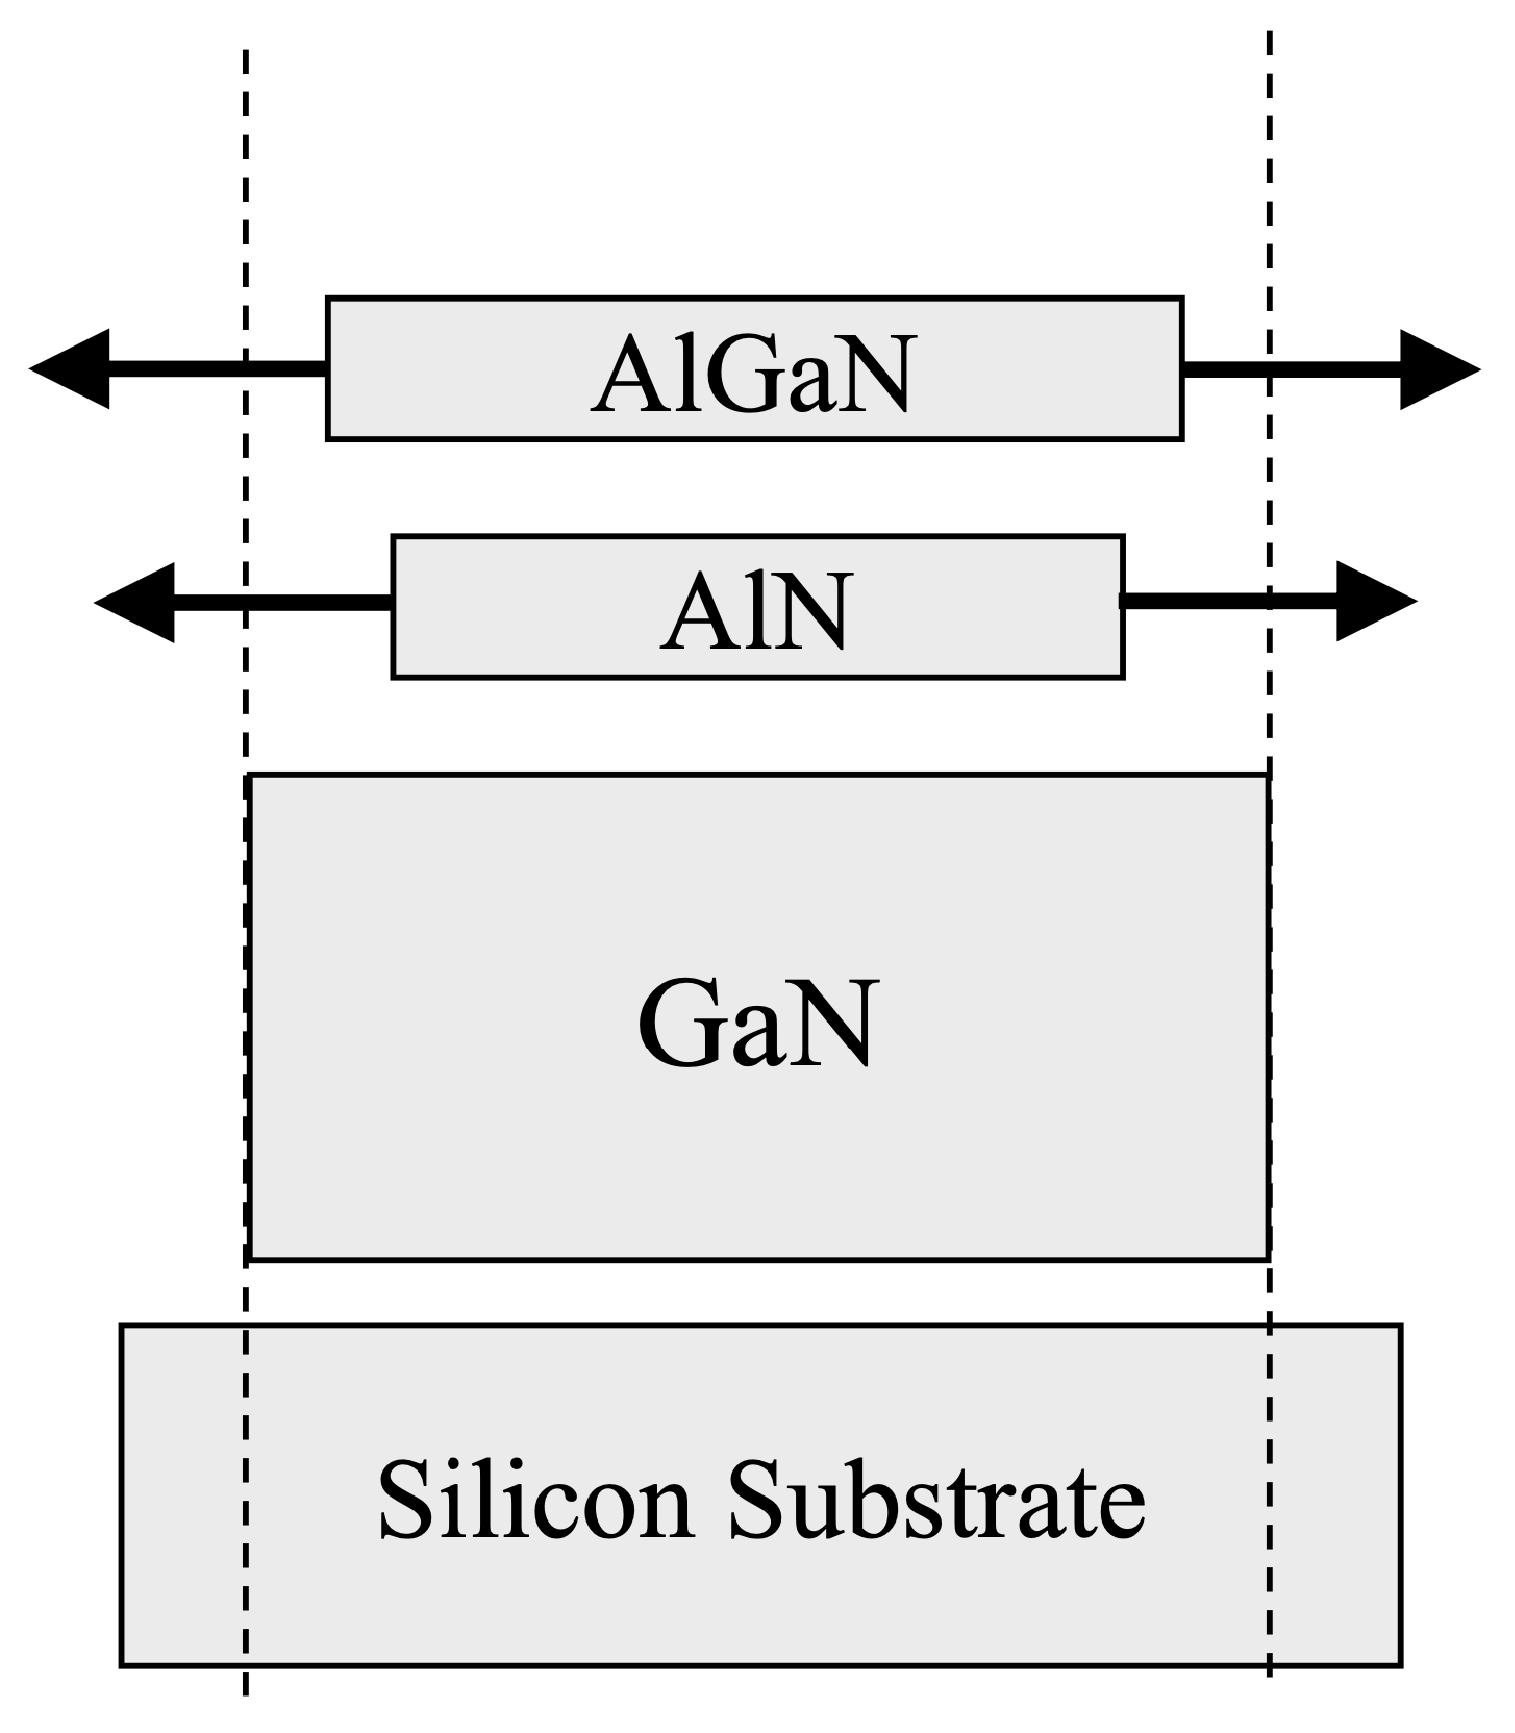
\includegraphics[width=0.6\textwidth]{ch2_8}
\caption[Thin film structure of AlGaN/AlN/GaN heterostructure]{Thin film structure of AlGaN/AlN/GaN heterostructure}
\label{fig:2.8}
\end{figure}

First we discuss the case where there is no external stress. In this case, the AlN film undergoes tensile \index{Elastic!strain} elastic strain, and its deformed lattice constant $a_{AlN}(epi)$ is equal to the lattice constant \index{Lattice!constant} $a_{GaN}$ of GaN, that is, $a_{AlN}(epi)=a_{GaN}$. Since the thickness of the AlN film is only 1 \unit{nm}, it can be reasonably approximated that the full lattice strain occurs in the AlN film. So the \index{Lattice!constant} lattice constant of the AlGaN film after deformation \index{Deformation} is equal to the lattice constant of the AlN film after the deformation, that is, $a_{AlGaN}(epi)=a_{AlN}(epi)$. Finally, we can approximately express the lateral lattice strain \index{Lattice!strain} of each layer of AlGaN/AlN/GaN \index{AlGaN/AlN/GaN heterojunction} heterojunction without external stress as follows:
\begin{equation}
S_{G a N}=\frac{a_{G a N}-a_{G a N}}{a_{G a N}}=0
\label{eq:2.13}
\end{equation}
\begin{equation}
S_{A l N}=\frac{a_{A l N}(e p i)-a_{A l N}}{a_{A l N}}=\frac{a_{G a N}-a_{A l N}}{a_{A l N}}
\label{eq:2.14}
\end{equation}
\begin{equation}
S_{AlGaN }=\frac{a_{A l G a N}(e p i)-a_{A l G a N}}{a_{A l G a N}}=\frac{a_{G a N}-a_{A l G a N}}{a_{A l G a N}}
\label{eq:2.15}
\end{equation}
In the ideal case of no external stress, the lattice deformations \index{Lattice!deformation} in the $x$ and $y$ directions of the AlN film and the AlGaN film are approximately the same, and the \index{Lattice!strain} lattice strain in the $z$ direction can be obtained according to the biaxial stress model \index{Biaxial stress model} described in \autoref{eq:2.10}.

In the presence of external stress, the lattice strain of each layer of \index{AlGaN/AlN/GaN heterojunction} AlGaN/AlN/GaN heterojunction will be more complicated. First, the GaN layer will deform laterally and longitudinally under the action of external stress, and the AlN film and AlGaN film will also deform accordingly. In this model, we approximately think that in the case of very weak external stress, each layer of the AlGaN/AlN/GaN heterojunction material still undergoes pure \index{Elastic!deformation} elastic \index{Deformation} deformation. The lattice constant \index{Lattice!constant} of the AlN film is still equal to that of the GaN layer, that is, the AlN film is still completely deformed. Therefore the lattice constant \index{Lattice!constant} of the deformed AlGaN film is still equal to that of the deformed AlN film. The mathematical expression is $a_{AlN}(starin)=a_{GaN}(starin)$, $a_{AlGaN}(starin)=a_{AlN}(starin)$. In this way, we can approximately express lateral lattice strain \index{Lattice!strain} of AlGaN/AlN/GaN heterojunction layers in the presence of external stress:
\begin{equation}
S_{G a N}(strain)=\frac{a_{G a N}(strain)-a_{G a N}}{a_{G a N}}
\label{eq:2.16}
\end{equation}
\begin{equation}
S_{A l N}(strain)=\frac{a_{A l N}(strain)-a_{A l N}}{a_{A l N}}=\frac{a_{G a N}(strain)-a_{A l N}}{a_{A l N}}
\label{eq:2.17}
\end{equation}
\begin{equation}
S_{AlGaN }(strain)=\frac{a_{A l G a N}(strain)-a_{A l G a N}}{a_{A l G a N}}=\frac{a_{G a N}(strain)-a_{A l G a N}}{a_{A l G a N}}
\label{eq:2.18}
\end{equation}

\begin{table}[H]
\renewcommand\arraystretch{1.5}
\centering
\caption[Physical parameters of wurtzite structure AlN and GaN]{Physical parameters of wurtzite structure AlN and GaN}
\setlength{\tabcolsep}{7mm}{
\begin{tabular}{cccc}
\hline \hline
Parameters                    & AlN     & GaN    & Ref           \\ \hline \hline
Lattice constant a (\unit{nm})     & 0.311   & 0.319  & \cite{vurgaftman2003band}     \\
Lattice constant c (\unit{nm})     & 0.498   & 0.519  & \cite{vurgaftman2003band}     \\
Bandgap $E_{g}$ (\unit{eV})        & 6.25    & 3.510  & \cite{vurgaftman2003band}     \\
Effective mass (Electron)     & 0.32    & 0.20   & \cite{vurgaftman2003band}     \\
Effective mass (Hole)         & 3.53    & 1.56   & \cite{bernardini1997spontaneous}     \\
Relative permittivity         & 8.5     & 10.4   & \cite{bernardini1997spontaneous}     \\
C11 (\unit{GPa})                   & 396     & 390    & \cite{vurgaftman2003band}     \\
C12 (\unit{GPa})                   & 137     & 145    & \cite{vurgaftman2003band}     \\
C13 (\unit{GPa})       			  & 108     & 106    & \cite{vurgaftman2003band}     \\
C33 (\unit{GPa})       			  & 373     & 398    & \cite{vurgaftman2003band}     \\
e31 (\unit{\coulomb\per\square\m})               & -0.58   & -0.452 & \cite{morkoc2008polarization,stevens2013thermo} \\
e33 (\unit{\coulomb\per\square\m})     		  & 1.55    & 0.818  & \cite{morkoc2008polarization,stevens2013thermo} \\
e311 (\unit{\coulomb\per\square\m})   			  & 5.850   & 6.185  & \cite{pal2011second}     \\
e333 (\unit{\coulomb\per\square\m})   			  & -10.750 & -8.090 & \cite{pal2011second}     \\
e133 (\unit{\coulomb\per\square\m})   			  & 4.533   & 1.543  & \cite{pal2011second}     \\
$P_{sp}$ (\unit{\coulomb\per\square\m})   			  & -0.081  & -0.029 & \cite{pal2011second}     \\ \hline \hline
\end{tabular}}
\label{tab:2.1}
\end{table}

\noindent In addition, under the action of external stress, the lattice deformations \index{Lattice!deformation} in the $x$ and $y$ directions of the GaN layer, AlN thin film, and AlGaN thin film \index{Thin film} may be different. Therefore, we can use the finite element analysis \index{Finite element analysis} method to calculate the \index{Strain} strain in the $x$, $y$ and $z$ directions of the GaN layer under the action of external stress according to the principles of material mechanics, and then calculate the $x$ and $y$ direction lattice constant \index{Lattice!constant} according to \autoref{eq:2.16}. On this basis, the lattice strains \index{Lattice!strain} in the $x$ and $y$ directions of the AlN film and the AlGaN film are solved respectively according to \autoref{eq:2.17} and \autoref{eq:2.18}. Finally, the lattice strain \index{Lattice!strain} in $z$ direction of the AlN film and the AlGaN film can be solved according to the biaxial \index{Biaxial stress model} stress model.

\subsection{Piezoelectric polarization charge of GaN AlGaN AlN layer}
\label{sec:Piezoelectric polarization charge of GaN AlGaN AlN layer}

In this subsection, we study the lattice strain \index{Lattice!strain} of the active region \index{Active region} of the \index{Cantilever} cantilevered GaN layer under the action of external stress using the methods of finite element \index{Finite element analysis} analysis. On this basis, the lattice strain and piezoelectric polarization charge \index{Piezoelectric!polarization charge} of GaN AlGaN AlN layer can be further obtained.

 According to the principles of material mechanics, we can solve the strain \index{Strain} of the cantilevered GaN under different external stresses through the methods of finite element analysis. \autoref{fig:2.9} shows the deformation \index{Deformation} of the GaN cantilever under 4 \unit{\mN} external stress simulated by COMSOL Multiphysics 5.1. The length, width, and height of the cantilever are 350 \unit{\um}, 60 \unit{\um}, and 4.3 \unit{\um}, respectively. The Poisson's ratio \index{Poisson's!ratio} and Young's modulus \index{Young's modulus} of the GaN material are 0.2 \cite{qin2017mechanical} and 290 \unit{GPa} \cite{ben2014young,nowak1999elastic} respectively. The external stress is applied to the front half of the \index{Cantilever} cantilever, and we set up a sampling point to extract the strain of the HEMT's active area.

\begin{figure}[H] 
\centering    
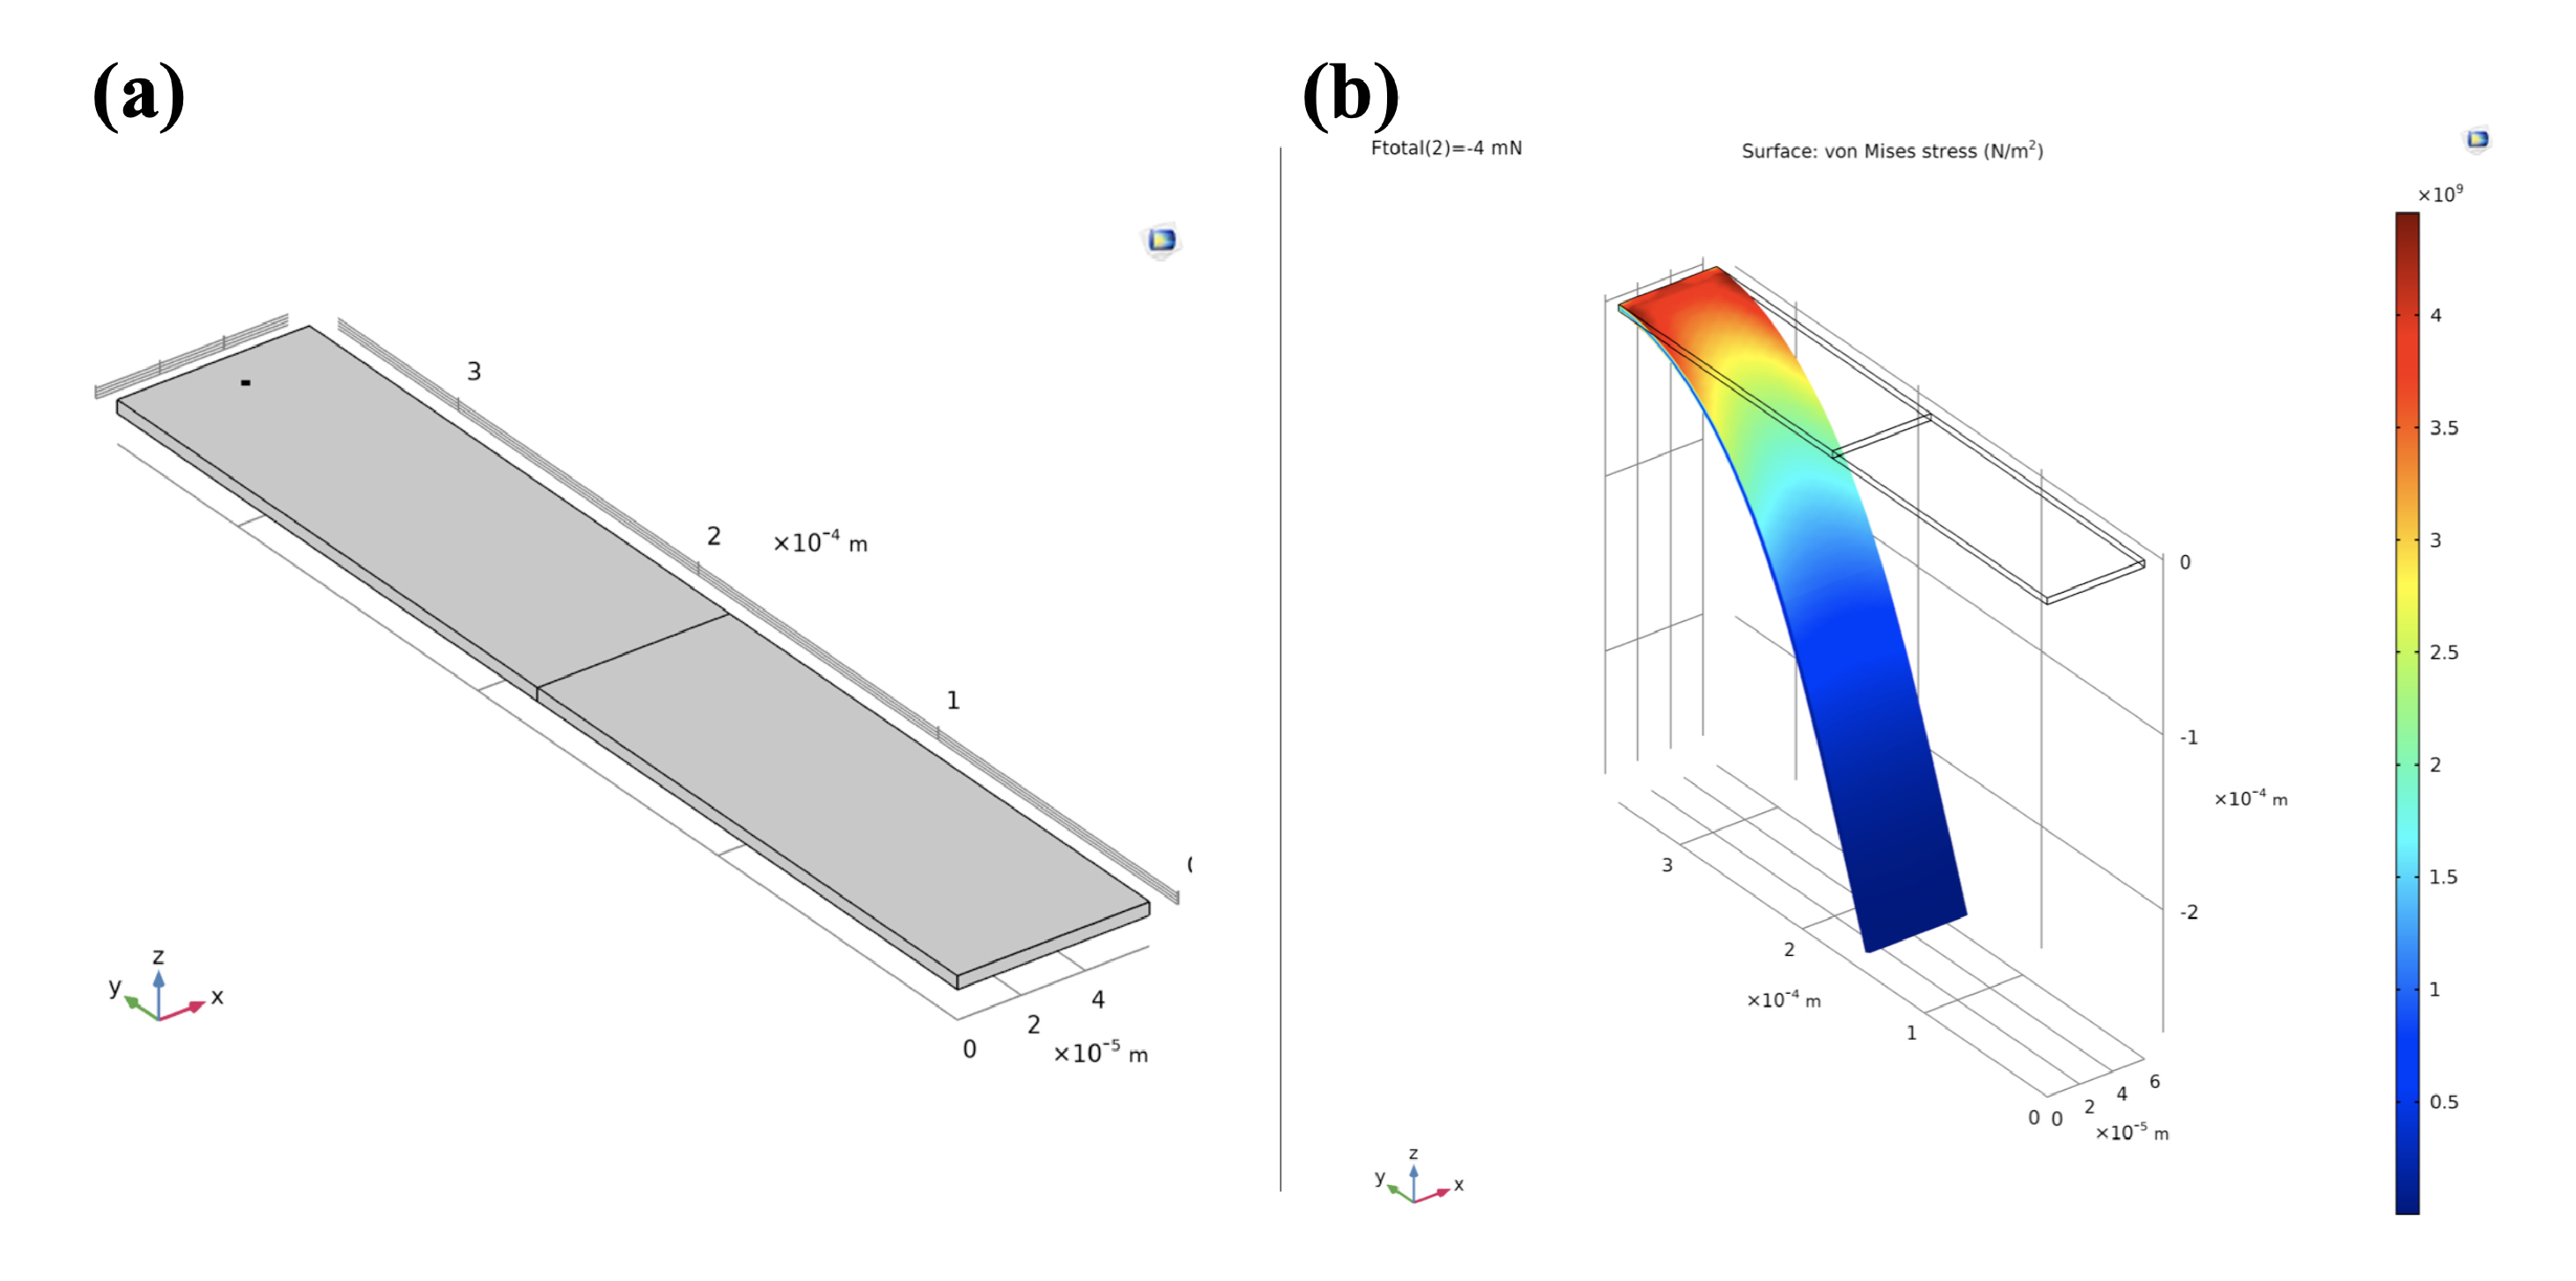
\includegraphics[width=0.9\textwidth]{ch2_9}
\caption[Finite element analysis of GaN cantilever strain under external stress]{Finite element analysis of GaN cantilever strain under external stress (a) Structure of the GaN cantilever. (b) Deformation of the GaN cantilever under 4 \unit{\mN} external stress.}
\label{fig:2.9}
\end{figure}

We take the theoretical calculation of the MPD \index{Magnetosensory power MEMS devices (MPD)} device in \autoref{ch:Magnetosensory Power Devices} in this thesis as an example. \autoref{fig:2.9}a is a schematic diagram of the structure of the \index{Cantilever} GaN cantilever, which is the same as that of the MPD cantilever. \autoref{fig:2.9}b shows the Von Mises stress \index{Von Mises stress} distribution of the GaN cantilever under 4 \unit{\mN} external stress. It can be seen that due to the special structure of the cantilever, the Von Mises stress at the fixed end of the cantilever is much larger than other regions, which is exactly the active region \index{Active region} of \index{AlGaN/AlN/GaN heterojunction} AlGaN/AlN/GaN heterojunction. So we verify that lattice strain \index{Lattice!strain} induced by external stress can be enlarged by the cantilever structure. By applying a downward normal force of 0 $\sim$ 24 \unit{\mN} to the front half of the cantilever, we calculated the GaN lattice strain \index{Lattice!strain} in the active region \index{Active region} corresponding to different external stresses. The calculation results are shown in \autoref{tab:2.2}. We can clearly see that under the action of external stress, the lattice strain in the $x$-direction of the active region is very small and almost negligible, while the lattice strain in the $y$-direction and $z$-direction is significant. Therefore, through the finite element analysis \index{Finite element analysis} model of material mechanics, we obtained the GaN's lattice strains in the $x$, $y$ and $z$ directions of \index{HEMT} cantilevered HEMT's active region under different external stresses, namely $𝑆_{xx}(GaN)$, $𝑆_{yy}(GaN)$ and $𝑆_{zz}(GaN)$. On this basis, the piezoelectric polarization charge \index{Piezoelectric!polarization charge} densities of GaN ($P_{GaN}^{PE}$), AlN ($P_{AlN}^{PE}$) and AlGaN ($P_{AlGaN}^{PE}$) thin films \index{Thin film} are further deduced, as shown in \autoref{tab:2.2}.

\begin{table}[]
\renewcommand\arraystretch{1.5}
\centering
\caption[Lattice strain of GaN cantilever active region and the corresponding piezoelectric polarization charge density of the films at 0 $\sim$ 24 \unit{\mN} downward force]{Lattice strain of GaN cantilever active region and the corresponding piezoelectric polarization charge density of the films at 0 $\sim$ 24 \unit{\mN} downward force}
\begin{tabular}{ccccccc}
\hline \hline
\multirow{2}{*}{\begin{tabular}[c]{@{}c@{}}F \\ (\unit{\mN})\end{tabular}} &
  \multirow{2}{*}{\begin{tabular}[c]{@{}c@{}}Strain tensor,\\ $S_{xx}$\end{tabular}} &
  \multirow{2}{*}{\begin{tabular}[c]{@{}c@{}}Strain tensor,\\ $S_{yy}$\end{tabular}} &
  \multirow{2}{*}{\begin{tabular}[c]{@{}c@{}}Strain tensor,\\ $S_{zz}$\end{tabular}} &
  \multicolumn{3}{c}{\begin{tabular}[c]{@{}c@{}}Piezoelectric polarization \\ charge densities (\unit{\coulomb\per\square\m})\end{tabular}} \\
    &            &           &            & $P_{GaN}^{PE}$  & $P_{AlN}^{PE}$  & $P_{AlGaN}^{PE}$  \\ \hline \hline
0   & 0          & 0         & 0          & 0       & -0.0492 & -0.0092 \\
-4  & -0.0001688 & 0.0148460 & -0.0036991 & -0.0097 & -0.0637 & -0.0200 \\
-8  & 0.0000291  & 0.0220201 & -0.0055929 & -0.0145 & -0.0710 & -0.0254 \\
-12 & 0.0001830  & 0.0268448 & -0.0068830 & -0.0178 & -0.0760 & -0.0291 \\
-16 & 0.0003008  & 0.0305848 & -0.0078887 & -0.0204 & -0.0798 & -0.0320 \\
-20 & 0.0003956  & 0.0337095 & -0.0087319 & -0.0226 & -0.0830 & -0.0344 \\
-24 & 0.0004726  & 0.0363812 & -0.0094546 & -0.0244 & -0.0857 & -0.0364 \\ \hline \hline
\end{tabular}
\label{tab:2.2}
\end{table}

So far, we have constructed a theoretical model of the \index{Piezoelectric!polarization charge} piezoelectric polarization charge intensity - external stress relationship ($P_{PE} - F$) of \index{MEMS} MEMS devices based on AlGaN/AlN/AlGaN \index{AlGaN/AlN/GaN heterojunction} heterojunction cantilever \index{Cantilever} structure. By combining piezoelectric constitutive \index{Piezoelectric!constitutive equation} equations, biaxial stress model \index{Biaxial stress model} and \index{Finite element analysis} finite element analysis, we can mathematically solve the piezoelectric polarization charge intensities of GaN ($P_{GaN}^{PE}$) layer, AlN ($P_{AlN}^{PE}$) layer and AlGaN ($P_{AlGaN}^{PE}$) layer when the cantilever is subjected to different external stresses $F$. The change of the piezoelectric polarization charge intensity $P_{PE}$ will affect the electrical properties of the heterojunction. In \autoref{sec:Self-consistent coupling model of strained AlGaN/AlN/GaN heterojunction}, we will study the modulation \index{Modulation} properties of the piezoelectric polarization charge intensity $P_{PE}$ on the AlGaN/AlN/AlGaN heterojunction energy \index{Energy band} band, carrier \index{Carrier!distribution} distribution, and 2DEG concentration \index{Two-dimensional electron gas (2DEG)} through a self-consistent coupled computational \index{Self-consistent computational model} model.

\section{Self-consistent coupling model of strained AlGaN/AlN/GaN heterojunction}
\label{sec:Self-consistent coupling model of strained AlGaN/AlN/GaN heterojunction}

\subsection{The theoretical equations of the model}
\label{sec:The theoretical equations of the model}

The physical model of the energy band \index{Energy band} of the \index{AlGaN/AlN/GaN heterojunction} AlGaN/AlN/GaN heterojunction is a semi-classical model based on the Schrödinger equation \index{Schrödinger equation} and the \index{Poisson's!equation} Poisson's equation. Under the effective mass approximation, the electron subband in the growth direction of the AlGaN/AlN/GaN heterojunction is the solution of the stationary Schrödinger equation \cite{lenka2011self}
\begin{equation}
-\frac{\hbar^{2}}{2} \frac{d}{d x}\left[\frac{1}{m^{*}} \frac{d \psi_{i}(x)}{d x}\right]+\left[V(x)-E_{i}\right] \psi_{i}(x)=0
\label{eq:2.19}
\end{equation}
where $m^{*}$ represents the effective mass of the electron at the edge of the conduction \index{Conduction band} band, $V(x)$ represents the potential energy, $E_{i}$ represents the energy of the ith subband, and $\psi_{i}(x)$ represents the wave function of the ith subband. Ignoring the non-parabolicity of the conduction band, we assume that  $m^{*}$ is independent of electron energy, which is isotropic and has abrupt changes at the interface \index{Interface} between AlGaN, AlN, and GaN.

The expression for potential \index{Potential!energy} energy $V(x)$ is:
\begin{equation}
\mathrm{V}(x)=V_{c}(x)+V_{h}(x)+V_{x c}(x)
\label{eq:2.20}
\end{equation}
where $V_{c}(x)$ represents the conduction band edge potential in the form of a step function related to the conduction band shift at the AlGaN/AlN/GaN heterojunction, and $V_{h}(x)$ is the Hartree potential \index{Hartree potential} induced by electrostatic interactions \index{Electrostatic!interactions} due to the distribution of mobile and stationary charges. $V_{x c}(x)$ is the exchange-correlated potential of many-body interactions that are not included in the \index{Hartree potential} Hartree potential \cite{lee2002self}.

$V_{h}(x)$ is the solution of the \index{Poisson's!equation} Poisson's equation:
\begin{equation}
\frac{d}{d x}\left[\varepsilon(x) \frac{d V_{h}(x)}{d x}\right]=-q \varphi(x)
\label{eq:2.21}
\end{equation}
where $\varepsilon(x)$ is the dielectric constant of the material with abrupt changes at the interface \index{Interface} between AlGaN, AlN and GaN. $q$ is the absolute value of the unit charge.

The total charge density distribution $\varphi(x)$ is given by:
\begin{equation}
\varphi(x)=\sum_{j=t, i, b} \sigma(x) \delta\left(x-x_{i}\right)+p(x)+N_{D}^{+}(x)-n(x)-N_{A}^{-}
\label{eq:2.22}
\end{equation}
where $\sigma(x)$ is the density of polarization charges \index{Polarization!charge} at the interface between AlGaN, AlN and GaN, $p(x)$ and $n(x)$ are the concentrations of holes and free electrons, respectively, and $N_{D}^{+}$ is the donor ion concentration, $N_{A}^{-}$ is the acceptor ion concentration.

According to the electrical neutrality \index{Electrical!neutrality condition} condition, this formula also must be satisfied in the AlGaN/AlN/GaN \index{AlGaN/AlN/GaN heterojunction} heterojunction interval:
\begin{equation}
\int_{x_{t}}^{x_{p}} \rho(x) d x=0
\label{eq:2.23}
\end{equation}
Written in the form of the sum of all charges:
\begin{equation}
\int_{x_{t}}^{x_{p}}\left[p(x)+N_{D}^{+}(x)-n(x)-N_{A}^{-}\right] d x=0
\label{eq:2.24}
\end{equation}
The carrier concentration \index{Carrier!concentration} distribution \index{Carrier!distribution} in the AlGaN/AlN/GaN heterojunction is given by:
\begin{equation}
n(x)=\sum_{i} n_{i}\left|\psi_{i}(x)\right|^{2}
\label{eq:2.25}
\end{equation}
where $n_{i}$ is the density of electrons in the ith subband, and usually expressed as a function of effective mass:
\begin{equation}
\mathrm{n}_{i}=\frac{m^{*} k_{B} T}{\pi \hbar^{2}} \ln \left[1+\exp \left(\frac{E_{F}-E_{i}}{k_{B} T}\right)\right]
\label{eq:2.26}
\end{equation}
$k_{B}$ and $T$ are Boltzmann constant and electron temperature, respectively.

The two-dimensional electron gas (2DEG) \index{Two-dimensional electron gas (2DEG)} areal density $N_{e}$ is equal to the sum of the electron densities in all the subbands of the heterojunction:
\begin{equation}
N_{e}=\int_{x_{t}}^{x_{b}} n(x) d x=\sum_{i} n_{i}
\label{eq:2.27}
\end{equation}

Next, we study the coupling of the \index{Piezoelectric!polarization charge} piezoelectric polarization charge intensity $P_{PE}$ under external \index{Strain} strain derived earlier into a self-consistent computational model \index{Self-consistent computational model} through the Poisson's equation \index{Poisson's!equation} of \autoref{eq:2.21}. Due to the non-centrosymmetric wurtzite \index{Wurtzite} crystal \index{Crystal} structure, there are two types of intrinsic polarizations in \index{AlGaN/AlN/GaN heterojunction} AlGaN/AlN/GaN heterojunctions \cite{ambacher1999two-b}: (i) spontaneous polarization \index{Spontaneous polarization} existing in AlGaN ($P_{AlGaN}^{sp}$), AlN ($P_{AlN}^{sp}$) and GaN ($P_{GaN}^{sp}$); (ii) piezoelectric polarization \index{Piezoelectric!polarization} due to lattice strain present in GaN ($P_{GaN}^{PE}$), AlN ($P_{AlN}^{PE}$) and AlGaN ($P_{AlGaN}^{PE}$). The density of polarization charges \index{Polarization!charge} at the \index{Interface} interface $P_{interface}$ of AlGaN, AlN and GaN can be expressed as:
\begin{equation}
P_{\text {Interface }}=P_{s p}+P_{P E}+e_{311} S_{\|}^{2}+e_{333} S_{\perp}^{2}+e_{313} S_{\|} S_{\perp}
\label{eq:2.28}
\end{equation}
where $P_{s p}$ is the spontaneous polarization charge intensity, $P_{P E}$ is the piezoelectric polarization charge intensity \index{Piezoelectric!polarization charge} induced by \index{Lattice!strain} lattice strain, and $e_{ijk}$ is the nonlinear \index{Piezoelectric!coefficient} piezoelectric coefficient. $S_{\perp}$ and $S_{\|}$ are the lattice strains perpendicular to c-plane and parallel to the c-plane induced by external stress, respectively. In this model, we only consider the piezoelectric polarization \index{Piezoelectric!polarization} effect in the linear case, so \autoref{eq:2.28} can be simplified as:
\begin{equation}
P_{\text {Interface }}=P_{s p}+P_{P E}
\label{eq:2.29}
\end{equation}
\autoref{eq:2.29} is the polarization charge density in the total charge density distribution of \autoref{eq:2.22}. The spontaneously polarized charge intensity of AlGaN (30$\%$ Al) can be given by \index{Vegard's law} Vegard's law \cite{vegard1921konstitution,denton1991vegard}:
\begin{equation}
P_{A l_{x} G a_{1-x} N}^{s p}=x P_{A l N}^{s p}+(1-x) P_{G a N}^{s p}-b_{A l_{x} G a_{1-x} N} x(1-x)
\label{eq:2.30}
\end{equation}
where $x$ is the percentage of Al composition in AlGaN and $b_{A l_{x} G a_{1-x} N}$ is the bending coefficient of AlGaN \cite{morkoc2008polarization}.

The above are the basic physics equations required to numerically solve the energy band \index{Energy band} of AlGaN/AlN/GaN heterojunction \index{AlGaN/AlN/GaN heterojunction} under external \index{Strain} strain \cite{morkoc2008polarization,lenka2011self,lenka20142deg,jiang2018thesis}.



\subsection{A self-consistent numerical method for one-dimensional Schrödinger-Poisson coupling equation}
\label{sec:A self-consistent numerical method for one-dimensional Schrodinger-Poisson coupling equation}

The analytical solution of the Schrödinger-Poisson coupling equation \index{Schrödinger-Poisson coupling equation} is difficult to derive, so it is usually solved by self-consistent \index{Self-consistent computational model} coupling numerical calculation using finite difference or finite element mathematical methods \cite{lenka2011self,lenka20142deg}, as shown in \autoref{fig:2.10}. First, we input the potential energy \index{Potential!energy} $V_{in}(x)$ as the initial iteration, and calculate the wave function $\psi_{i}(x)$ and the corresponding eigenenergy $E_{i}$ using the steady-state Schrödinger wave equation (\autoref{eq:2.19}), and then use the \autoref{eq:2.25} and \autoref{eq:2.16} to calculate the electron density $n_{i}$ and the carrier concentration distribution \index{Carrier!concentration} $n(x)$ in the subband. The Hartree potential \index{Hartree potential} $V_{h}(x)$ is further calculated in the Poisson's equation \index{Poisson's!equation} using the given donor concentration $N^{+}_{D}(x)$, acceptor concentration $N_{A}^{-}$, and polarization charge density \index{Polarization!charge} at the \index{Interface} interface $\sigma(x)$, and the potential \index{Potential!energy} energy $V_{x}$ is also calculated according to \autoref{eq:2.20}. Then We substitute the obtained potential energy $V_{x}$ at this time into the steady-state Schrodinger wave equation to find the new wave function $\psi_{i}(x)$ and the corresponding eigenenergy $E_{i}$, and to solve the new carrier concentration distribution $n(x)$. This new $n(x)$ together with the donor concentration and acceptor concentration can be used to calculate the new Hartree potential \index{Hartree potential} $V_{h}(x)$ and new potential energy \index{Potential!energy} $V_{x}$ in the \index{Poisson's!equation} Poisson's equation. Compare the newly obtained potential energy $V_{x}$ with the previous result, and if it is outside the error range, continue to iterate until convergence is achieved. Finally, the self-consistent solutions of $V_{x}$ and $n(x)$ are used to further determine the \index{Energy band} energy band diagram and the carrier concentration \index{Carrier!concentration} of the \index{AlGaN/AlN/GaN heterojunction} AlGaN/AlN/GaN heterojunction.

\begin{figure}[H] 
\centering    
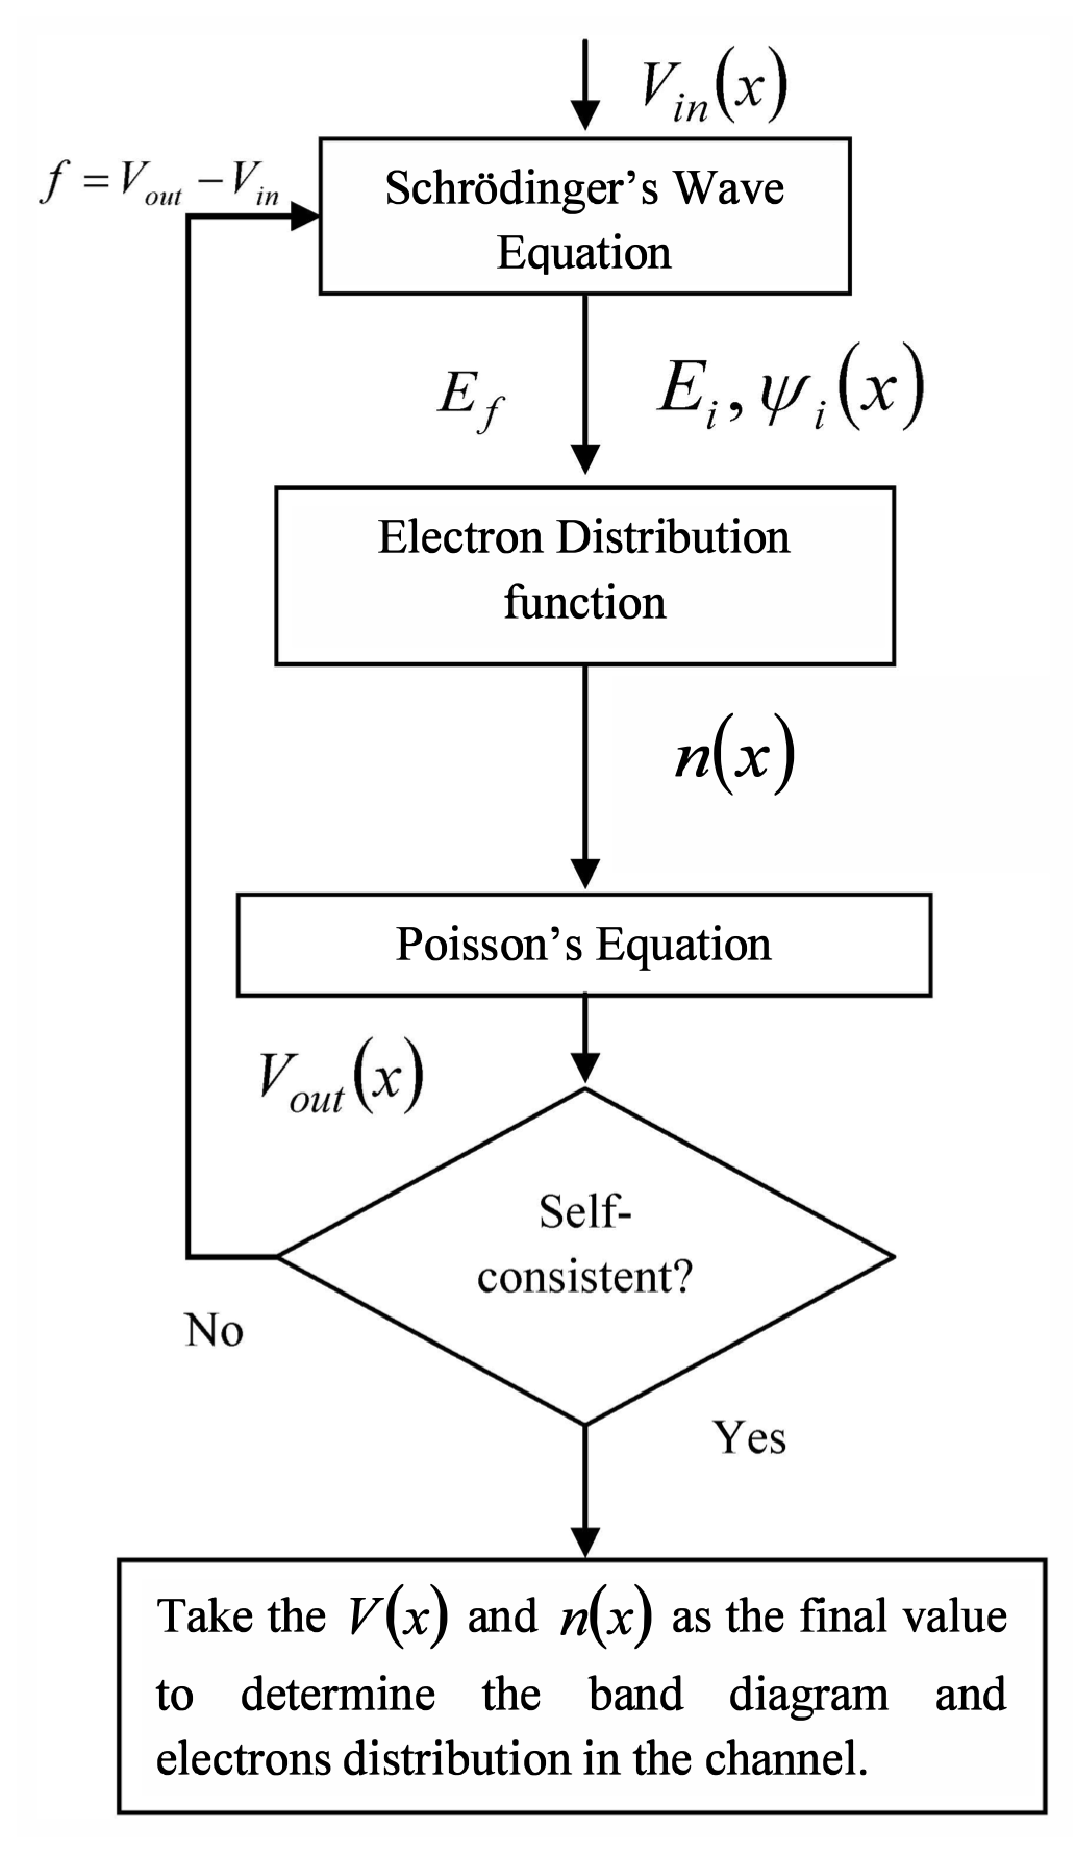
\includegraphics[width=0.6\textwidth]{ch2_10}
\caption[Iteration process of Schrodinger-Poisson self-consistent calculation]{Iteration process of Schrodinger-Poisson self-consistent calculation \protect\cite{lenka20142deg}}
\label{fig:2.10}
\end{figure}

\section{The framework of theoretical model}
\label{sec:The framework of theoretical model}

\begin{figure}[H] 
\centering    
\includegraphics[width=0.9\textwidth]{ch2_11}
\caption[Framework diagram of the theoretical model]{Framework diagram of the theoretical model}
\label{fig:2.11}
\end{figure}

So far, we have constructed a complete theoretical model of the MEMS device based on the \index{AlGaN/AlN/GaN heterojunction} AlGaN/AlN/AlGaN heterojunction cantilever \index{Cantilever} structure. By combining the piezoelectric constitutive \index{Piezoelectric!constitutive equation} equation, the biaxial stress model \index{Biaxial stress model} and the finite element \index{Finite element analysis} analysis, we deduce the mathematical relationship between the piezoelectric polarization charge intensity \index{Piezoelectric!polarization charge} and the external stress. Through the self-consistent coupling calculation model \index{Self-consistent computational model} of the AlGaN/AlN/GaN heterojunction, we further solved the modulation \index{Modulation} effect of the piezoelectric polarization charge intensity at the interface on the heterojunction energy band \index{Energy band} and the electron-hole wave function, thus successfully constructing a semi-classical physical model to explain the regulation mechanism \index{Physical!mechanism} of external stress on the electrical properties of MEMS devices. The overall framework \index{Physical!framework} of the theoretical model is shown in \autoref{fig:2.11}. The piezoelectric polarization charge density \index{Piezoelectric!polarization charge} at the interface is effectively modulated by external stress, thereby changing the electrostatic field \index{Electrostatic!field} in the \index{AlGaN/AlN/GaN heterojunction} AlGaN/AlN/GaN heterojunction, and finally modulating the heterojunction energy band, electron-hole wave function and carrier \index{Carrier!distribution} distribution. This model is an approximate semi-classical physical model with series of simplifications and approximations, which successfully reveals the modulation \index{Modulation} characteristics of piezotronics \index{Piezotronics} effect on MEMS \index{MEMS} devices based on AlGaN/AlN/AlGaN heterojunction cantilever \index{Cantilever} structure.

\section{Simulation results of theoretical model}
\label{sec:Simulation results of theoretical model}

In the above theoretical analysis, we mainly take the theoretical modeling of MEMS under the downward force as an example to illustrate the method. Theoretical modeling and analysis of upward forces is similar. Different from the previous downward stress situation, the upward force on the cantilever \index{Cantilever} weakens the electrical performance of MEMS, that is, the reaction will increase the potential well at the AlN/GaN \index{Interface} interface, thereby reducing the concentration of \index{Two-dimensional electron gas (2DEG)} 2DEG. \autoref{tab:2.3} shows the lattice strain \index{Lattice!strain} of GaN cantilever \index{Cantilever} active region \index{Active region} and the corresponding piezoelectric polarization charge density \index{Piezoelectric!polarization charge} of the films at 0 $\sim$ 24 \unit{\mN} upward force. The corresponding simulation results of \index{Magnetosensory power MEMS devices (MPD)} MPD is in \autoref{fig:ch2_MPD_theory_up}.

\begin{table}[H]
\renewcommand\arraystretch{1}
\centering
\caption[Lattice strain of GaN cantilever active region and the corresponding piezoelectric polarization charge density of the films at 0 $\sim$ 24 \unit{\mN} upward force]{Lattice strain of GaN cantilever active region and the corresponding piezoelectric polarization charge density of the films at 0 $\sim$ 24 \unit{\mN} upward force}
\begin{tabular}{ccccccc}
\hline \hline
\multirow{2}{*}{\begin{tabular}[c]{@{}c@{}}F \\ (\unit{\mN})\end{tabular}} &
  \multirow{2}{*}{\begin{tabular}[c]{@{}c@{}}Strain tensor,\\ $S_{xx}$\end{tabular}} &
  \multirow{2}{*}{\begin{tabular}[c]{@{}c@{}}Strain tensor,\\ $S_{yy}$\end{tabular}} &
  \multirow{2}{*}{\begin{tabular}[c]{@{}c@{}}Strain tensor,\\ $S_{zz}$\end{tabular}} &
  \multicolumn{3}{c}{\begin{tabular}[c]{@{}c@{}}Piezoelectric polarization \\ charge densities (\unit{\coulomb\per\square\m})\end{tabular}} \\
    &            &           &            & $P_{GaN}^{PE}$  & $P_{AlN}^{PE}$  & $P_{AlGaN}^{PE}$  \\ \hline \hline
0   & 0          & 0         & 0          & 0       & -0.0492 & -0.0092 \\
4  & 0.0003518 & -0.0152836 & 0.0037110 & 0.0099 & -0.0340 & 0.0021 \\
8  & 0.0002443  & -0.0226277 & 0.0055619 & 0.0148 & -0.0267 & 0.0076 \\
12 & 0.0001342  & -0.0274473 & 0.0067851 & 0.0180 & -0.0219 & 0.0111 \\
16 & 0.0000447  & -0.0311016 & 0.0077137 & 0.0204 & -0.0183 & 0.0138 \\
20 & -0.0000288  & -0.0341114 & 0.0084785 & 0.0224 & -0.0153 & 0.0161 \\
24 & -0.0000895  & -0.0366690 & 0.0091278 & 0.0240 & -0.0128 & 0.0179 \\ \hline \hline
\end{tabular}
\label{tab:2.3}
\end{table}


\begin{figure}[H] 
\centering    
\includegraphics[width=0.88\textwidth]{ch2_MPD_theory_up}
\caption[Simulation results of MPD with upward magnetic force]{Simulation results of MPD with upward magnetic force}
\label{fig:ch2_MPD_theory_up}
\end{figure}

\begin{figure}[H] 
\centering    
\includegraphics[width=0.88\textwidth]{ch2_MPD_theory_down}
\caption[Simulation results of MPD with downward magnetic force]{Simulation results of MPD with downward magnetic force}
\label{fig:ch2_MPD_theory_down}
\end{figure}


\begin{figure}[H] 
\centering    
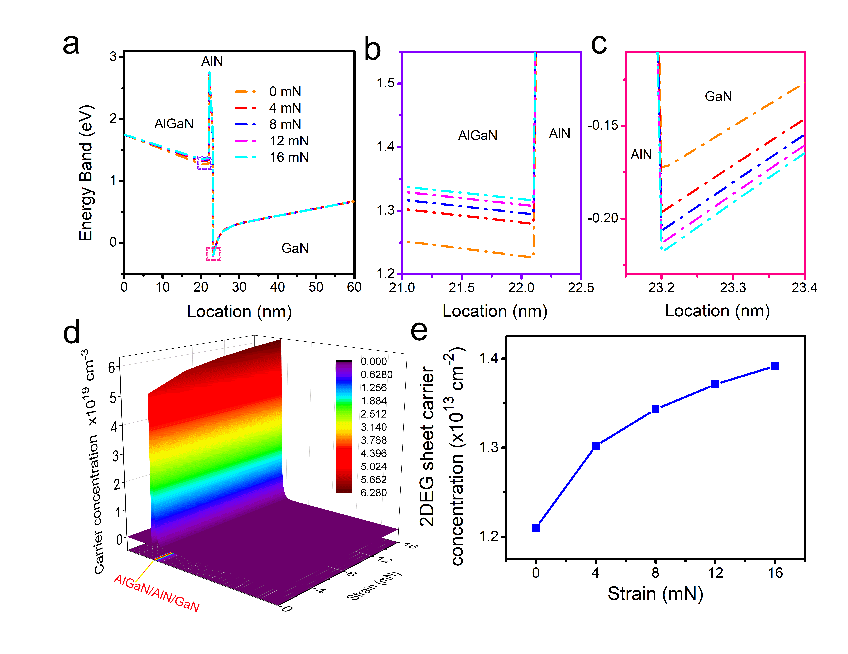
\includegraphics[width=0.9\textwidth]{ch2_SPD_theory}
\caption[Simulation results of SPD with downward normal force]{Simulation results of SPD with downward normal force}
\label{fig:ch2_SPD_theory}
\end{figure}


We also present the theoretical simulation results of the \index{Strain-controlled power MEMS devices
(SPD)} SPD and MPD \index{Magnetosensory power MEMS devices (MPD)} at downward force, as shown in \autoref{fig:ch2_SPD_theory} and \autoref{fig:ch2_MPD_theory_down}. The detailed analysis can be found in \autoref{ch:Strain-controlled power devices} and \autoref{ch:Magnetosensory Power Devices}. By comparing with the experimental test, it can be concluded that the model successfully verifies the experimental results of SPD and MPD, and reveals the physical mechanism \index{Physical!mechanism} of MEMS \index{MEMS} devices based on AlGaN/AlN/GaN \index{AlGaN/AlN/GaN heterojunction} heterojunction cantilever \index{Cantilever} structure.

Furthermore, we use the established model to simulate the \index{Energy band} energy band and \index{Carrier!distribution} carrier distribution characteristics of \index{MEMS} MEMS devices with different cantilever \index{Cantilever} lengths under the control of 0 $\sim$ 24 \unit{\mN} downward stress, as shown in \autoref{fig:2.400}, \autoref{fig:2.450} and \autoref{fig:2.500}. The corresponding cantilever \index{Cantilever} lengths are 400 \unit{\um}, 450 \unit{\um} and 500 \unit{\um}, and the width and thickness are 60 \unit{\um} and 4.3 \unit{\um}. In these figures, Figure (a) is the \index{AlGaN/AlN/GaN heterojunction} AlGaN/AlN/GaN heterojunction \index{Conduction band} conduction band; Figure (b) is the enlarged conduction band \index{Conduction band} of AlGaN/AlN and AlN/GaN \index{Potential!well} potential well; Figure (c) is the enlarged conduction band of AlN/GaN potential \index{Potential!well} well; Figure (d) is the \index{Carrier!distribution} carrier\index{Carrier!concentration} concentration distribution; Figure (e) is the two-dimensional electron gas (2DEG) \index{Two-dimensional electron gas (2DEG)} areal density. It can be clearly seen that under the same external stress, the AlN/GaN wells of \index{MEMS} MEMS devices with cantilever \index{Cantilever} lengths of 450 \unit{\um} (\autoref{fig:2.450}c) and 500 \unit{\um} (\autoref{fig:2.500}c) are deeper than that of 400 \unit{\um} (\autoref{fig:2.400}c). So compared with the MEMS with shorter \index{Cantilever} cantilever, more carriers are bound in the potential well \index{Potential!well} of MEMS with longer cantilever \index{Cantilever} (\autoref{fig:2.400}d, \autoref{fig:2.450}d and \autoref{fig:2.500}d), and the two-dimensional electron gas (2DEG) areal density in the MEMS with cantilever length of 450 \unit{\um} (\autoref{fig:2.450}e) and 500 \unit{\um} (\autoref{fig:2.500}e) are all higher than that of  400 \unit{\um} (\autoref{fig:2.400}e). Based on the theoretical simulation results, we can design cantilevers \index{Cantilever} with different lengths and structures to modulate the MEMS's sensitivity to the external stress response. Therefore, the theoretical model can provide theoretical guidance for the development of MEMS cantilever \index{Cantilever} devices based on AlGaN/AlN/GaN heterojunctions.

\begin{figure}[H] 
\centering    
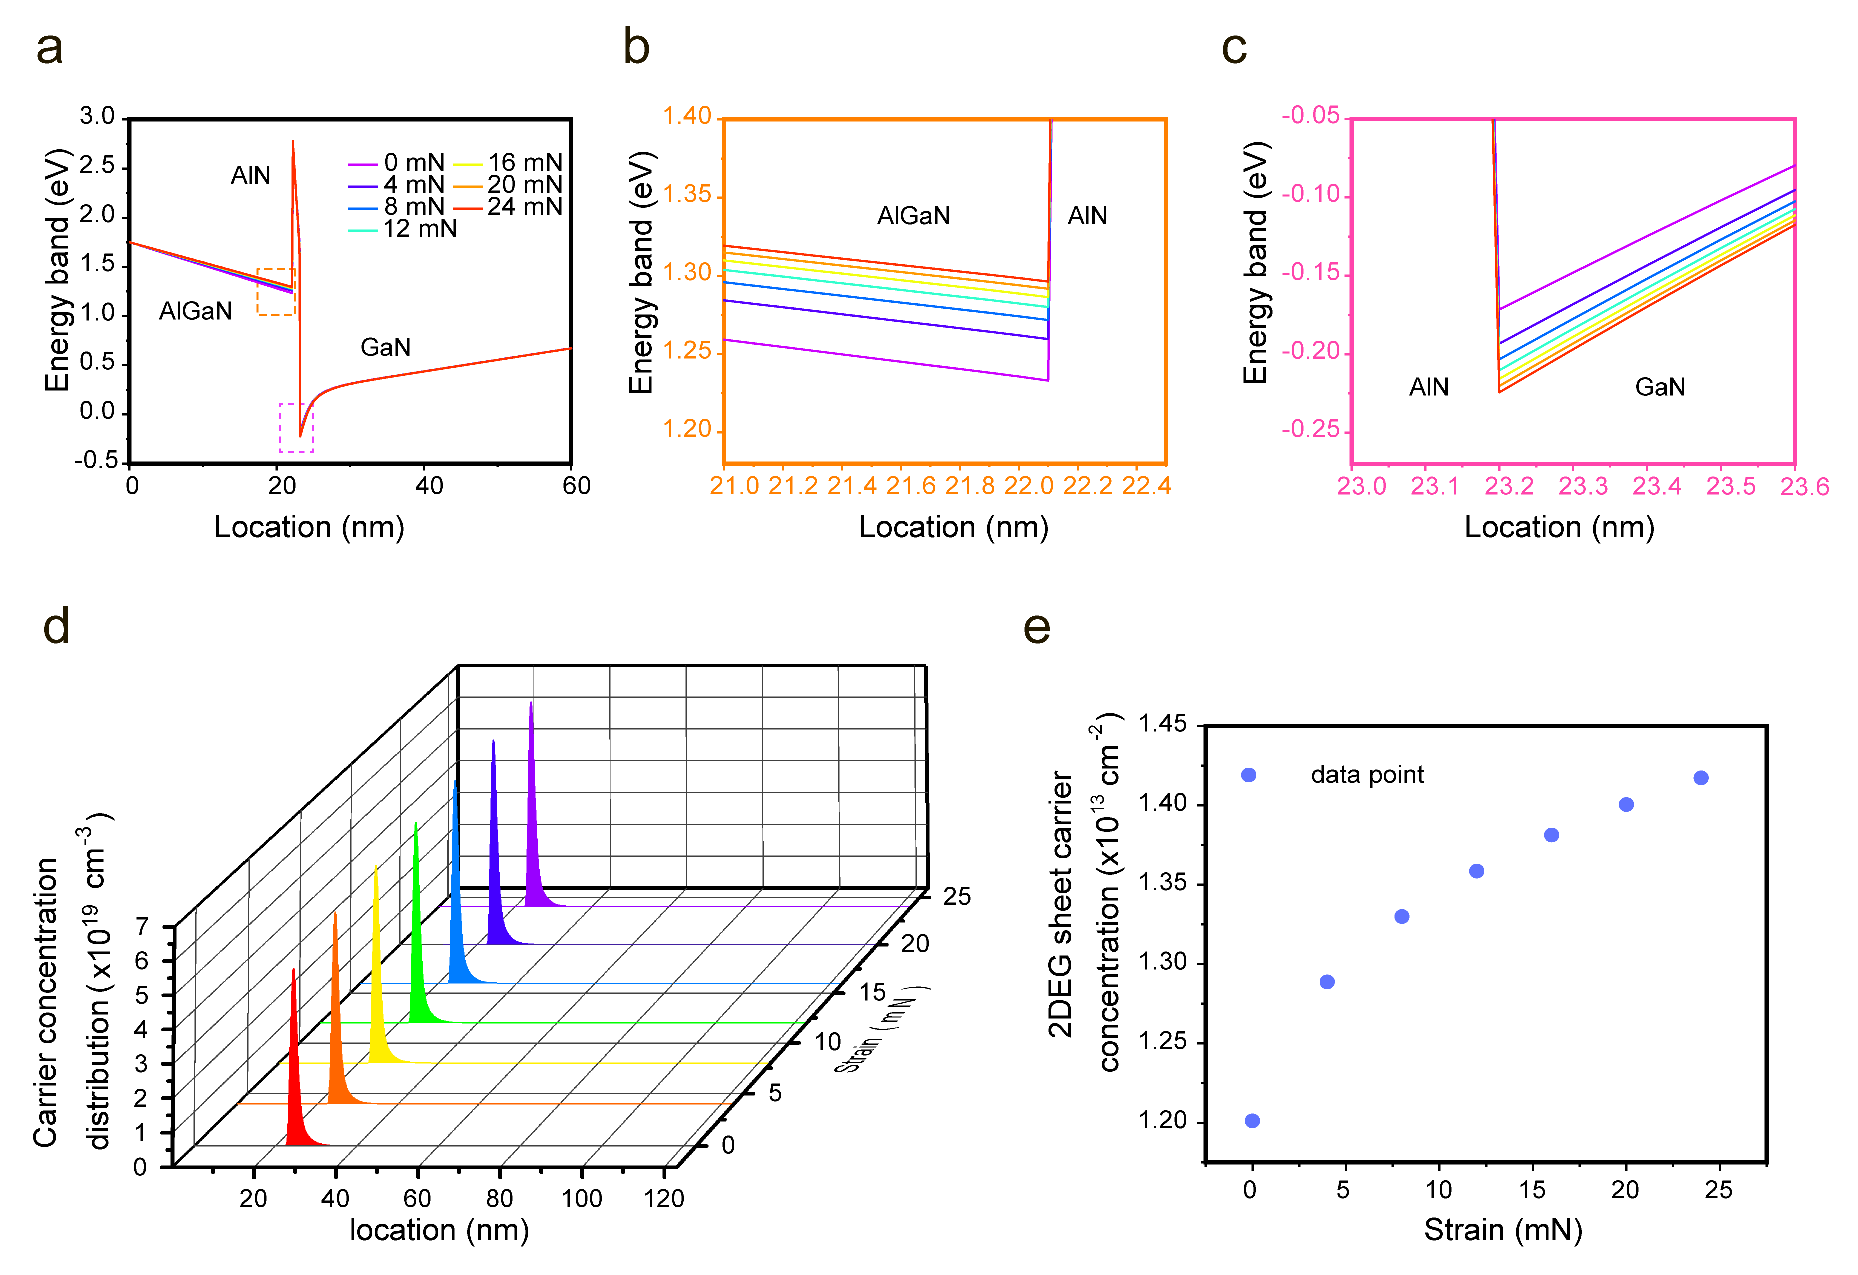
\includegraphics[width=0.9\textwidth]{ch2_400}
\caption[Simulation results of MEMS with the cantilever length of 400 \unit{\um} under downward force]{Simulation results of MEMS with the cantilever length of 400 \unit{\um} under downward force}
\label{fig:2.400}
\end{figure}

\begin{figure}[H] 
\centering    
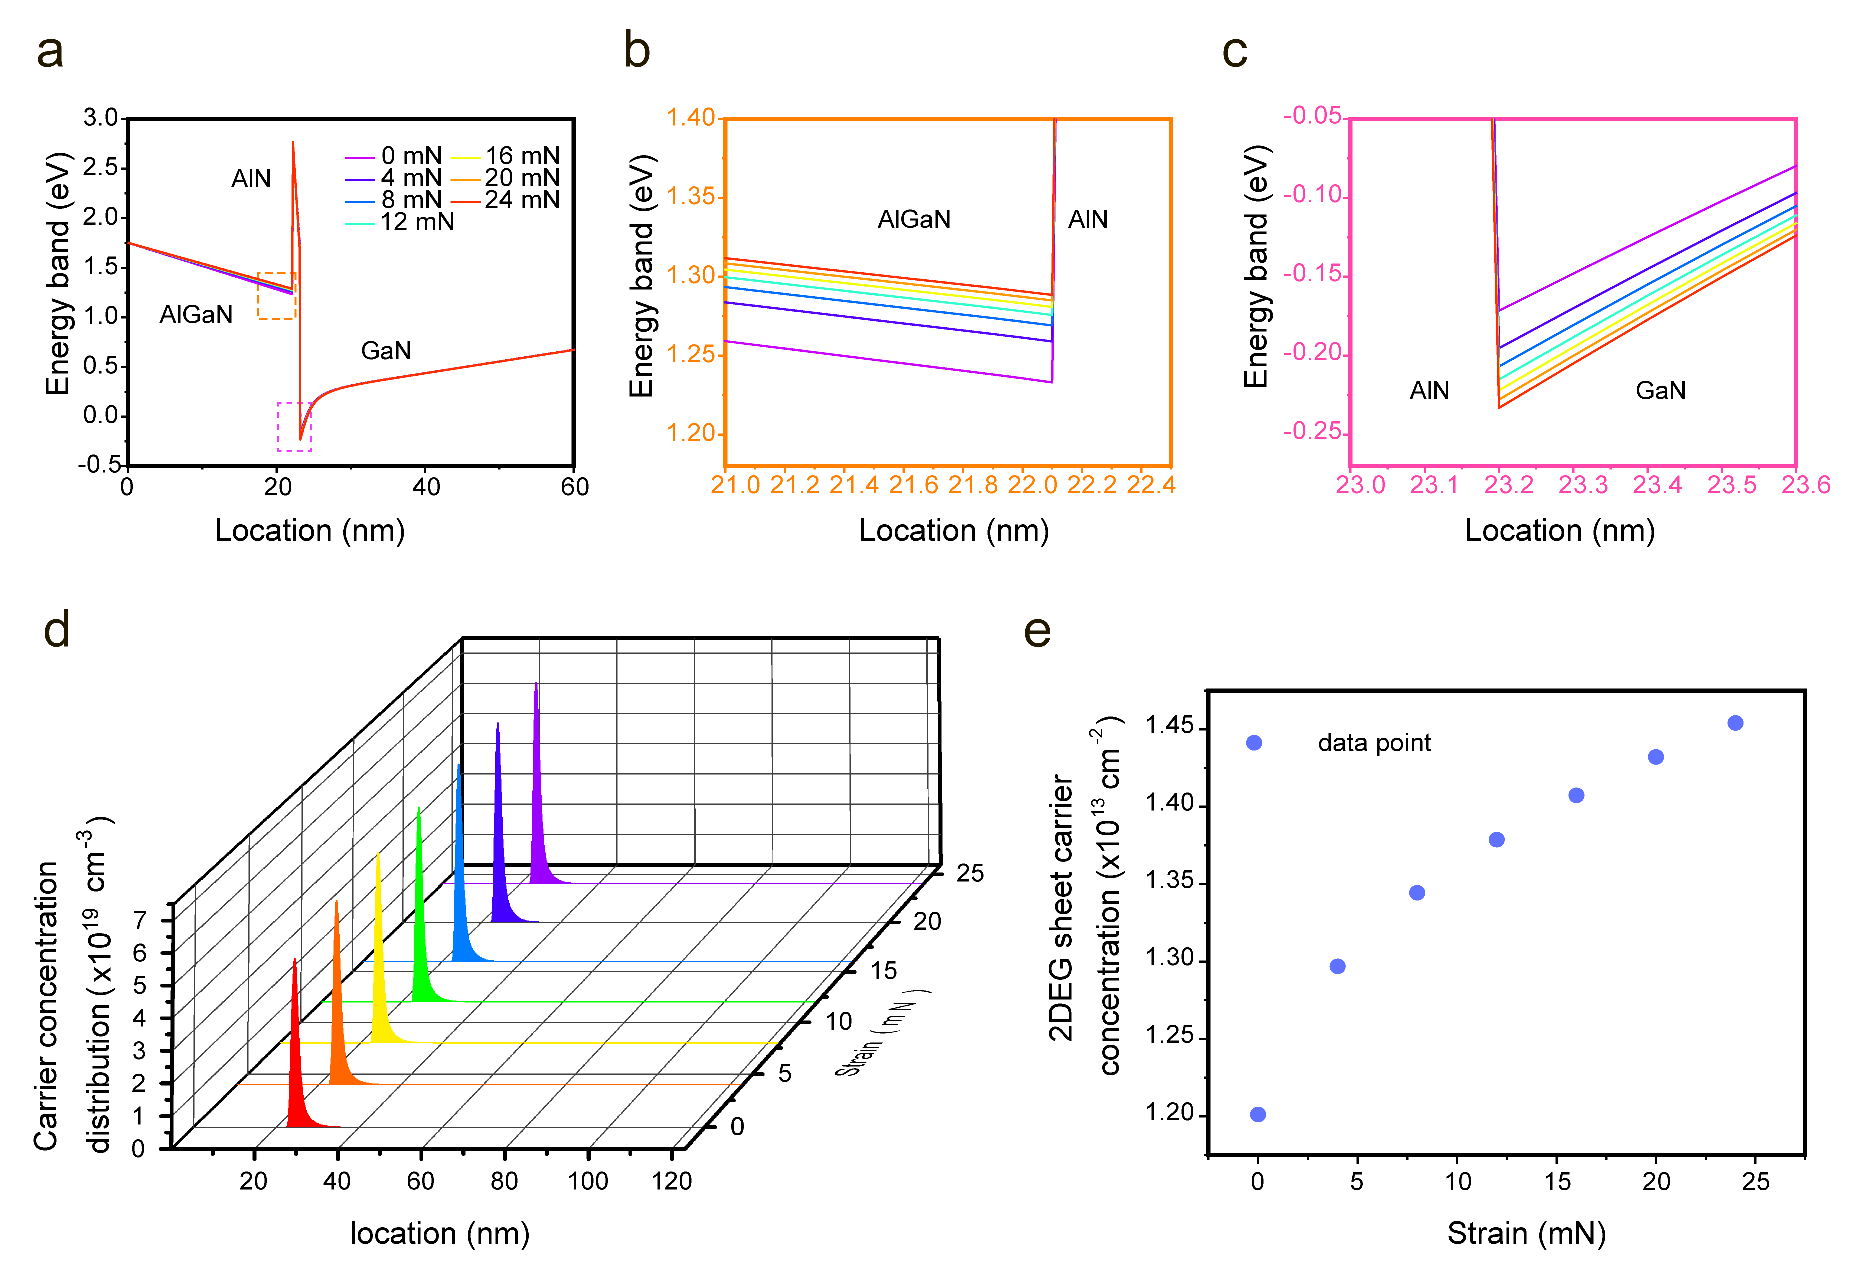
\includegraphics[width=0.85\textwidth]{ch2_450}
\caption[Simulation results of MEMS with the cantilever length of 450 \unit{\um} under downward force]{Simulation results of MEMS with the cantilever \index{Cantilever} length of 450 \unit{\um} under downward force}
\label{fig:2.450}
\end{figure}

\begin{figure}[H] 
\centering    
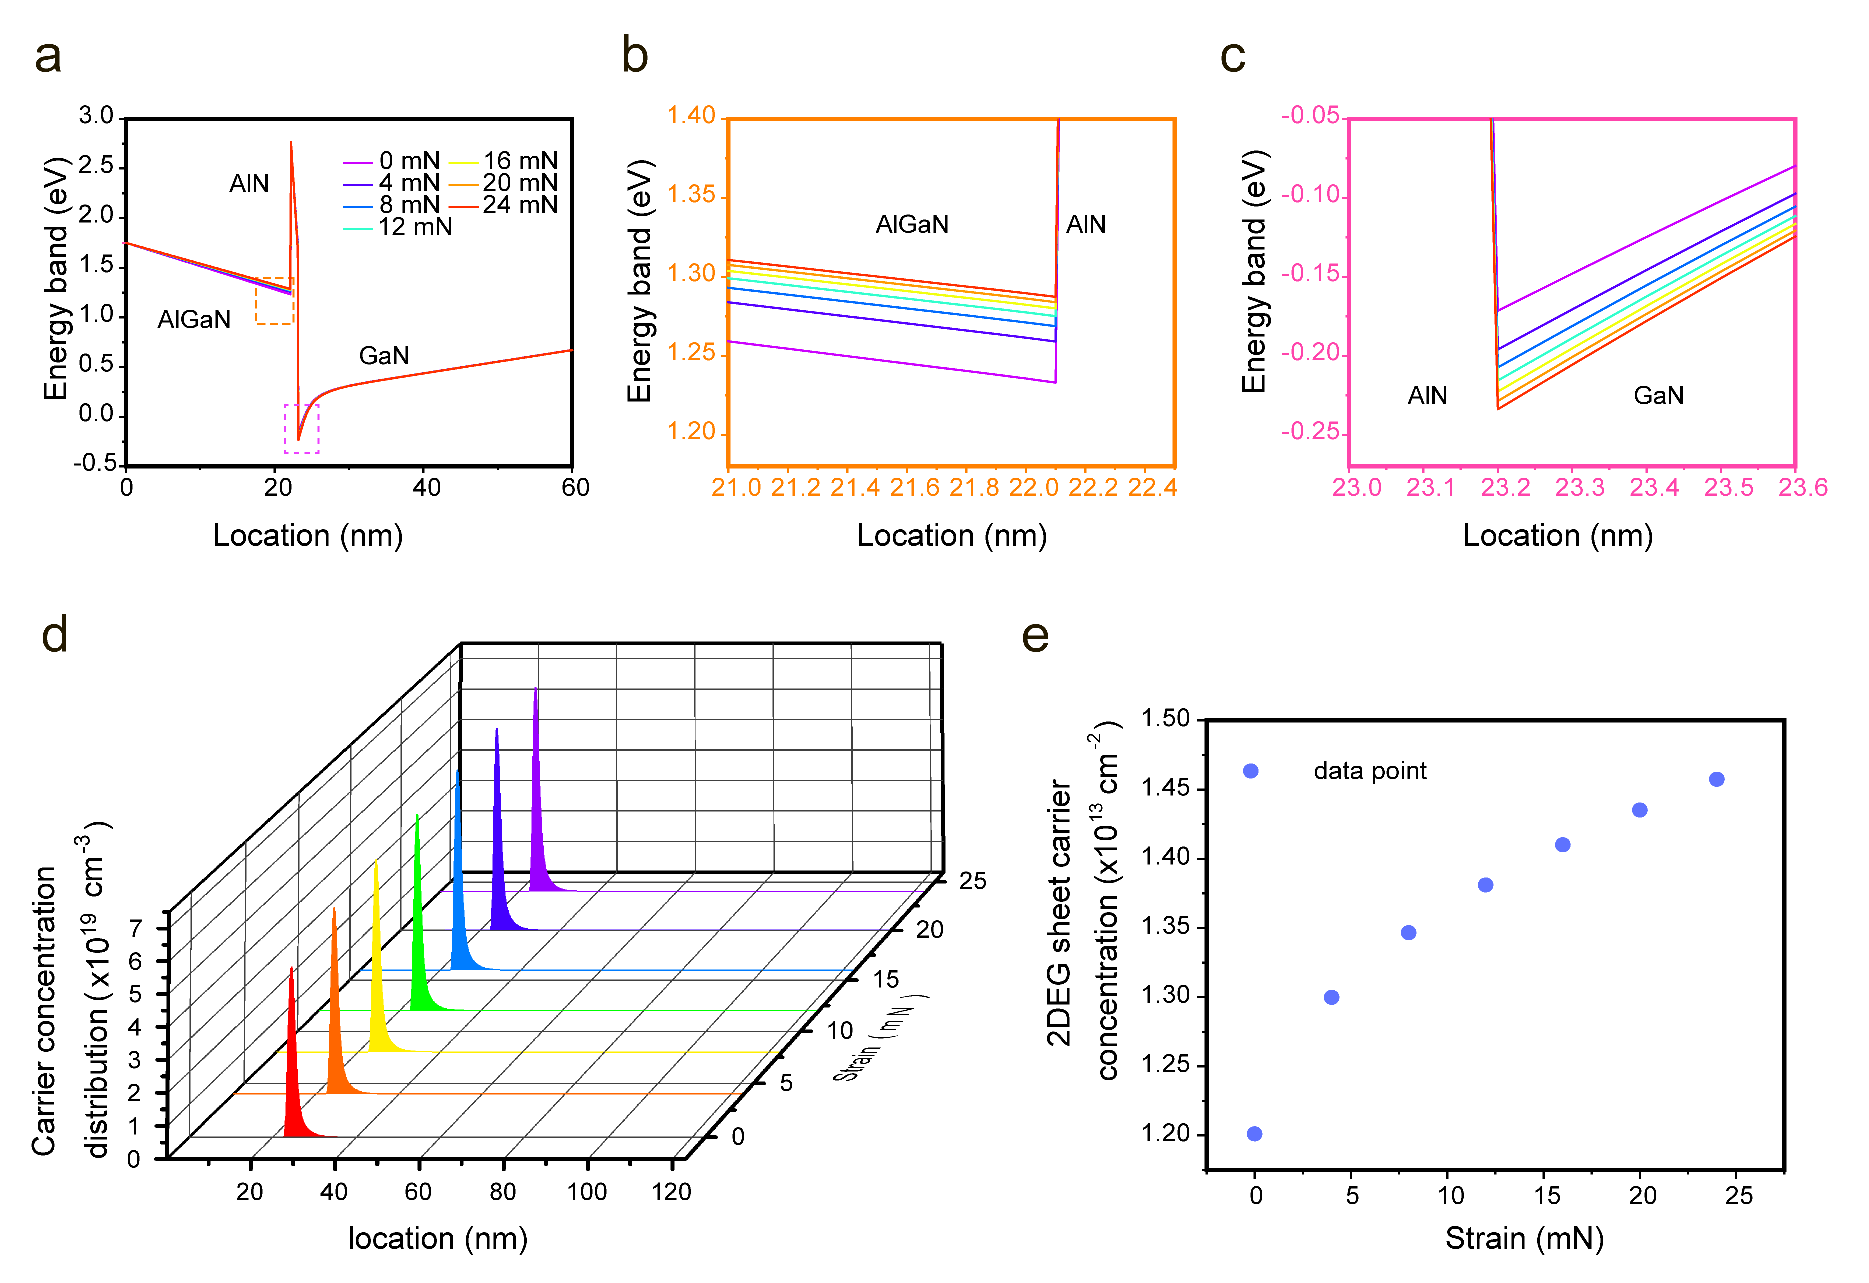
\includegraphics[width=0.85\textwidth]{ch2_500}
\caption[Simulation results of MEMS with the cantilever length of 500 \unit{\um} under downward force]{Simulation results of MEMS with the cantilever length of 500 \unit{\um} under downward force}
\label{fig:2.500}
\end{figure}

\section{Summary}
In this study, a semi-classical physical model of the MEMS \index{MEMS} device with a cantilever \index{Cantilever} structure based on AlGaN/AlN/GaN heterojunction was established by using piezoelectric theory. The mathematical relationship between the lattice strain \index{Lattice!strain} and the piezoelectric polarization charge \index{Piezoelectric!polarization charge} of the multilayer heterojunction film was deduced through piezoelectric constitutive equation \index{Piezoelectric!constitutive equation} and \index{Biaxial stress model} biaxial stress model. Then the finite element analysis \index{Finite element analysis} method of material mechanics was used to calculate the piezoelectric polarization charge intensity \index{Piezoelectric!polarization charge} of the heterojunction film under different external stresses, and the one-dimensional Schrödinger-Poisson self-consistent coupling model was used to calculate the modulation \index{Modulation} characteristics of the external stress on the energy band of the AlGaN/AlN/GaN heterojunction \index{AlGaN/AlN/GaN heterojunction} and the electrical properties of the \index{MEMS} MEMS device. The theoretical results successfully verify the experimental results of the new MEMS devices designed and fabricated in this paper, namely SPD and MPD. The model provides theoretical guidance for the development of novel MEMS cantilever \index{Cantilever} devices based on \index{AlGaN/AlN/GaN heterojunction} AlGaN/AlN/GaN heterojunctions.

\nomenclature{$P_{PE}$}{Piezoelectric polarization charge density}
\nomenclature{$P_{Psp}$}{Spontaneous polarization charge density}
\nomenclature{$P_{GaN}^{PE}$}{Piezoelectric polarization charge density of GaN}
\nomenclature{$P_{AlGaN}^{PE}$}{Piezoelectric polarization charge density of AlGaN}
\nomenclature{$P_{AlN}^{PE}$}{Piezoelectric polarization charge density of AlN}
\nomenclature{$P_{GaN}^{sp}$}{Spontaneous polarization charge density of GaN}
\nomenclature{$P_{AlN}^{sp}$}{Spontaneous polarization charge density of AlN}
\nomenclature{$P_{AlGaN}^{sp}$}{Spontaneous polarization charge density of AlGaN}
\nomenclature{$Al_{x}Ga_{1-x}N$}{The percentage of AlN in AlGaN}
\nomenclature{$b_{A l_{x} G a_{1-x} N}$}{Bending coefficient of AlGaN}
\nomenclature{$e_{ijk}$}{Nonlinear piezoelectric coefficient of GaN crystal}
\nomenclature{$S_{\perp}$}{Lattice strains perpendicular to c-plane of GaN crystal}
\nomenclature{$S_{\|}$}{Lattice strains parallel to c-plane of GaN crystal}
\nomenclature{$k_{B}$}{Boltzmann constant}
\nomenclature{$T$}{Electron temperature}
\nomenclature{$N_{e}$}{Sum of the electron densities in all the subbands}
\nomenclature{$\boldsymbol{E}$}{Electric field strength vector}
\nomenclature{$\boldsymbol{D}$}{Electric displacement vector}
\nomenclature{$\sigma$}{Stress tensor}
\nomenclature{$\boldsymbol{c}_{E}$}{Elastic coefficient tensor}
\nomenclature{$\boldsymbol{e}$}{Linear piezoelectric coefficient}
\nomenclature{$\boldsymbol{k}$}{Dielectric constant tensor}
\nomenclature{$\boldsymbol{S}$}{Strain tensor}
\nomenclature{$P_{interface}$}{The density of polarization charges at the interface}
\nomenclature{$n_{i}$}{Density of electrons in the ith subband}
\nomenclature{$S_{x x}, S_{x}$}{Strains in the $x$ direction}
\nomenclature{$S_{y y}, S_{y}$}{Strains in the $y$ direction}
\nomenclature{$S_{z z}, S_{z}$}{Strains in the $z$ direction}
\nomenclature{$\varepsilon_{0}$}{Vacuum permittivity}
\nomenclature{$\mathbf{P}$}{Electric polarization strength}
\nomenclature{$P_{z}$}{Piezoelectric polarization in the $z$ direction}
\nomenclature{$v$}{Poisson's ratio}

\nomenclature{$a_{AlGaN}$}{Lattice constant of AlGaN}
\nomenclature{$a_{AlN}$}{Lattice constant of AlN}
\nomenclature{$a_{GaN}$}{Lattice constant of GaN}


\nomenclature{$N_{D}^{+}$}{Donor ion concentration}
\nomenclature{$n(x)$}{Concentrations of free electrons}
\nomenclature{$p(x)$}{Concentrations of holes}

\nomenclature{$\varepsilon(x)$}{Dielectric constant AlGaN, AlN and GaN}
\nomenclature{$N_{A}^{-}$}{Acceptor ion concentration}
\nomenclature{$q$}{Absolute value of the unit charge}

\nomenclature{$V_{c}(x)$}{Conduction band edge potential}
\nomenclature{$V_{h}(x)$}{Hartree potential}
\nomenclature{$V_{x c}(x)$}{Exchange-correlated potential}

\nomenclature{$S_{B}$}{Stain of the thin film $B$}

\nomenclature{$a_{A}$}{Lattice constant of the substrate $A$}
\nomenclature{$a_{B}(epi)$}{Lattice constant of the thin film $B$}
\nomenclature{$a_{AlN}(strain)$}{Lattice constant of strained AlN}
\nomenclature{$a_{GaN}(strain)$}{Lattice constant of strained GaN}
\nomenclature{$a_{AlGaN}(strain)$}{Lattice constant of strained AlGaN}
\nomenclature{$S_{AlN}(strain)$}{Strain of strained AlN}
\nomenclature{$S_{GaN}(strain)$}{Strain of strained GaN}
\nomenclature{$S_{AlGaN}(strain)$}{Strain of strained AlGaN}
\nomenclature{$a$}{Lattice constant}
\nomenclature{$c$}{Lattice constant}
\nomenclature{$E_{g}$}{Bandgap energy}
\nomenclature{$e31$}{Piezoelectric Constant}
\nomenclature{$e33$}{Piezoelectric Constant}
\nomenclature{$e311$}{Piezoelectric Constant}
\nomenclature{$e333$}{Piezoelectric Constant}
\nomenclature{$e133$}{Piezoelectric Constant}
\nomenclature{$C11$}{Elastic constants}
\nomenclature{$C12$}{Elastic constants}
\nomenclature{$C13$}{Elastic constants}
\nomenclature{$C33$}{Elastic constants}

\nomenclature{$𝑆_{xx}(GaN)$}{Strain of GaN in the $x$ direction}
\nomenclature{$𝑆_{yy}(GaN)$}{Strain of GaN in the $y$ direction}
\nomenclature{$𝑆_{zz}(GaN)$}{Strain of GaN in the $z$ direction}
\nomenclature{$m^{*}$}{Effective mass of the electron}
\nomenclature{$V(x)$}{Potential energy}
\nomenclature{$E_{i}$}{Energy of the ith subband}
\nomenclature{$\psi_{i}(x)$}{Wave function of the ith subband}


\nomenclature[z-GaN]{GaN}{Gallium nitride}
\nomenclature[z-AlN]{AlN}{Aluminum nitride}
\nomenclature[z-AlGaN]{AlGaN}{Aluminium gallium nitride}
\nomenclature[z-AlN]{HEMT}{High-electron-mobility transistor}
\nomenclature[z-2DEG]{2DEG}{The two-dimensional electron gas}
\nomenclature[z-AlN]{FET}{Field effect transistor}